\documentclass[11pt]{article}
% Match the US Letter page and 1.08-inch margins of main (3).pdf.
\usepackage[letterpaper,margin=1.08in]{geometry}
\usepackage[T1]{fontenc}
\usepackage{microtype}
\usepackage{amsmath,amssymb,amsthm}
\usepackage{tikz}
\usepackage[hidelinks]{hyperref}

% All sections share these environments and counters.
\newtheorem{lemma}{Lemma}[section]
\newtheorem{proposition}[lemma]{Proposition}
\newtheorem{theorem}[lemma]{Theorem}
\newtheorem{auxlemma}{Lemma}[section]
\renewcommand{\theauxlemma}{\thesection.\Alph{auxlemma}}
\theoremstyle{definition}
\newtheorem{fact}{Fact}[section]
\newtheorem{remark}[lemma]{Remark}
\newtheorem{definition}{Definition}[section]
\numberwithin{equation}{section}
\setlength{\emergencystretch}{2em}

\usepackage[nameinlink,noabbrev]{cleveref}
\crefname{fact}{Fact}{Facts}
\Crefname{fact}{Fact}{Facts}
\crefname{auxlemma}{Lemma}{Lemmas}
\Crefname{auxlemma}{Lemma}{Lemmas}
\crefname{definition}{Definition}{Definitions}
\Crefname{definition}{Definition}{Definitions}
\crefname{theorem}{Theorem}{Theorems}
\Crefname{theorem}{Theorem}{Theorems}
\crefname{proposition}{Proposition}{Propositions}
\Crefname{proposition}{Proposition}{Propositions}

\title{Strict hot spots and absence of interior critical points on smooth
simply connected planar domains}
\author{George Coote with GPT 6.1 Sol}
% Date of the supplied manuscript.
\date{September 24, 2026}

\begin{document}
\maketitle
\begin{abstract}
This manuscript presents a readability revision of a proposed proof of
the strict hot spots conjecture for smooth bounded simply connected planar
domains. The claimed result is that every nonzero eigenfunction for the
first positive Neumann eigenvalue has nonvanishing gradient in the
interior, so all its global maxima and minima lie on the boundary,
including when the eigenvalue is multiple. George Coote worked with
GPT 6.1 Sol to expand and clarify the supplied argument so that he and
other readers can review it with less effort. This revision does not
constitute independent verification of the claimed result.
\end{abstract}

\section{Introduction}\label{sec:introduction}

This document revises the exposition of a proposed proof in the supplied
manuscript. George Coote's purpose in working with GPT 6.1 Sol was to make
that argument readable enough for him and others to examine its
mathematical validity without having to reconstruct numerous omitted
steps. The main statements and proof strategy were already present in
the supplied text. The revision expands definitions, calculations,
references, and logical transitions; it does not claim that Coote
originated the result or its proof, or that the proposed proof has been
independently verified. The following introduction describes the claim
and the argument presented for it.

The hot-spots problem arose from Rauch's discussion of the long-time
behavior of heat flow with insulating boundary conditions \cite{Rau75}.
Its spectral formulation asks whether the extrema of a first-positive
Neumann eigenfunction occur on the boundary. Ba\~nuelos and Burdzy
distinguished strict and nonstrict formulations, and assertions about
every eigenfunction from the existence of one favorable eigenfunction
\cite{BanuelosBurdzy}. These distinctions matter when the eigenvalue is multiple.

Let $\Omega\subset\mathbb R^2$ be a nonempty bounded simply connected open
set with $C^\infty$ boundary. In particular, $\Omega$ is connected. Set
\begin{equation}\label{eq:first-neumann-eigenvalue}
 \lambda_N=\inf_{\substack{0\ne v\in H^1(\Omega;\mathbb R)\\
                            \int_\Omega v=0}}
 \frac{\int_\Omega|\nabla v|^2}{\int_\Omega v^2},
\end{equation}
and let $V$ be the real Neumann eigenspace for $\lambda_N$.
This is the first positive eigenvalue; sources that count the constant
eigenfunction first call it the second Neumann eigenvalue.

The supplied manuscript claims the following theorem.
\begin{samepage}
\begin{theorem}\label[theorem]{thm:strict-hot-spots}
For every $0\ne u\in V$,
\[
 \nabla u(x)\ne0\qquad(x\in\Omega).
\]
In particular,
\begin{equation}\label{eq:strict-hot-spots}
 \min_{y\in\partial\Omega}u(y)<u(x)<\max_{y\in\partial\Omega}u(y)
 \qquad(x\in\Omega).
\end{equation}
\end{theorem}
\end{samepage}

The theorem imposes no convexity or symmetry condition. It applies to
every member of the first positive eigenspace, including when the
eigenvalue is multiple. The nonvanishing-gradient conclusion also rules
out interior saddle points.

\paragraph{Background and methods.}
Topology matters in the hot-spots problem. Burdzy and Werner constructed
a planar counterexample with two holes and a simple first-positive
eigenvalue \cite{BW99}. Bass and Burdzy obtained examples with both extrema
strictly in the interior \cite{BB00}, and Burdzy subsequently obtained
this behavior with just one hole \cite{Bur05}. The simply connected
planar conjecture is stated explicitly in \cite[Conjecture 1.2(ii)]{Bur05}.

Several geometric special cases already establish strong gradient
conclusions. Jerison and Nadirashvili proved a positive directional
derivative for every first-positive eigenfunction on convex planar domains
with two orthogonal reflection symmetries, allowing multiple eigenvalues
\cite[Theorem 1.4]{JN00}. Probabilistic coupling methods developed by
Ba\~nuelos and Burdzy \cite{BanuelosBurdzy} led to further results. Pascu
proved boundary-only extrema for antisymmetric eigenfunctions on
$C^{1,\alpha}$ convex planar domains with one reflection symmetry, where
$0<\alpha<1$ \cite{Pas02}. Atar and Burdzy treated every first-positive
eigenfunction on lip domains, a class of Lipschitz domains bounded between
graphs of functions with Lipschitz constants at most one \cite{AB04}.
Miyamoto obtained interior critical-point exclusion under a
spectral-diameter condition, giving nonsymmetric nearly circular convex
examples \cite[Lemma 1.2 and Theorem A]{Miy07}.

For polygons, Siudeja proved hot-spots results for a class of acute
triangles \cite{Siu15}. Judge and Mondal, with their subsequent erratum,
excluded interior critical points for every first-positive Neumann
eigenfunction on every Euclidean triangle \cite{JM20,JM22}. Chen, Gui and
Yao established the finer classification of nonvertex critical points
\cite{CGY26}. These results concern domains with corners;
\cref{thm:strict-hot-spots} concerns smooth simply connected planar domains.

Recent quantitative work measures how far the hot-spots conclusion can
fail. For general bounded connected Lipschitz domains, de Dios Pont, Hsu
and Taylor determined the sharp dimension-dependent upper bound for the
ratio of a first-positive Neumann eigenfunction's supremum over the domain
to its maximum on the boundary \cite[Definition 1 and Theorem 4]{dDPHT25}.
Deng, Jiang and Yang obtained quantitative bounds for convex domains in
two-dimensional space forms \cite{DJY26}. Such ratios concern extrema;
excluding every interior critical point also requires excluding saddle points.

The supplied proof starts from Rohleder's variational principle for tangent vector
fields \cite{Rohleder,Roh24}. In its lip-domain application, taking
componentwise absolute values after a suitable rotation preserves the
required tangent boundary condition and yields directional monotonicity.
Its argument uses scalar boundary multipliers to keep tangency on an
arbitrary smooth boundary, constructing those multipliers through a
reciprocal Green-kernel theorem.

Each Cartesian derivative of an eigenfunction solves the same Helmholtz
equation, but its boundary values need not have a fixed sign. The Neumann
condition constrains the two derivatives together: their vector is tangent
to the boundary. The argument uses that constraint through a nonnegative quadratic
form on tangent boundary data. Its nullspace consists exactly of the
boundary traces of first-positive eigenfunction gradients. The kernel
construction supplies scalar boundary multipliers that preserve this nullspace if an
interior critical point exists.

\paragraph{The mechanism.}
Write $\mathbb D=\{z\in\mathbb C:|z|<1\}$ and $S^1=\partial\mathbb D$,
and let $\Phi:\overline{\mathbb D}\to\overline\Omega$ be a smooth
conformal parametrization. For a tangent vector field $X$, the
divergence--curl energy $Q(X)$ is at least $\lambda_N\|X\|_2^2$, with equality
exactly for gradients of functions in $V$; see \cref{prop:vector-variational}.
After the conformal change of variables, solving the scalar Helmholtz
equation in each fixed Cartesian component extends Lipschitz boundary
data $h:S^1\to\mathbb R^2$ to a vector field $X_h$ on $\Omega$.
For tangent data, the quadratic form
\[
 E(h)=Q(X_h)-\lambda_N\|X_h\|_2^2
\]
is nonnegative, and it vanishes exactly when $X_h=\nabla v$ for some
$v\in V$. Here tangency at $s$ means tangency to $\partial\Omega$ at
$\Phi(s)$. For a nonzero eigenfunction $u\in V$, put
$g(s)=\nabla u(\Phi(s))$. This is the gradient in the coordinates of
$\Omega$, parametrized on the circle. Its extension is $X_g=\nabla u$,
so $E(g)=0$, and a real Lipschitz scalar multiplier $b$ satisfies
\[
 E(bg)=\frac12\iint_{S^1\times S^1}
 N(s,t)(b(s)-b(t))^2g(s)\cdot g(t)\,ds\,dt.
\]
Here $N$ is a symmetric boundary kernel, strictly positive off the
diagonal, and the corresponding interior
evaluation kernel is denoted by $K$; see \cref{prop:multiplier-identity}.

The sign of $g(s)\cdot g(t)$ prevents a direct positivity argument in
this identity. The kernel theorem supplies multipliers whose squared
differences remove the factor $N$. For every interior point $p$,
\[
 D_p(s,t)=\frac{K(p,s)K(p,t)}{N(s,t)}\quad(s\ne t),
 \qquad D_p(s,s)=0,
\]
is conditionally negative semidefinite. \Cref{lem:hilbert-embedding}
constructs a separable real Hilbert space and an injective Lipschitz map
$b$ from the circle into that space, with squared distances $D_p$.
The construction uses the positive anchored kernel, a quotient by the
zero-norm subspace, and completion; the kernel estimates give injectivity
and the Lipschitz bound. Applying the energy identity to the coordinates
$b_j$ of $b$ in an orthonormal basis, and justifying the sum by dominated
convergence, gives
\[
 \sum_j E(b_jg)=\frac12|\nabla u(\Phi(p))|^2.
\]
At a critical point every nonnegative summand vanishes. The equality case
then gives $v_j\in V$ with boundary gradient $b_jg$. If the set
$S_g=\{s:g(s)\ne0\}$ is dense in the circle, injectivity of $b$ produces
three linearly independent eigenfunctions, contradicting
\cref{prop:multiplicity}. If $S_g$ is not dense, the gradients vanish
on an open boundary arc. Two independent eigenfunctions then have a
nonzero linear combination with both zero value and zero normal
derivative on that arc. Its local extension by zero solves the Helmholtz
equation across the arc, and interior uniqueness gives the contradiction.

The construction of $D_p$ is the central analytic step. It first
regularizes the disk Green function so that the entrywise reciprocal of
every finite kernel matrix has at most one positive eigenvalue. This
property survives successive rank-one updates along columns of the
current kernel matrix, which sum the Green resolvent over a finite set of
integration nodes. Positive quadrature and monotone limits then pass from
those matrices to the singular Green kernel and finally to its boundary
kernels. Taking the boundary limit before removing a compact-support
cutoff avoids treating a Poisson kernel as an $L^2$ function when it need
not be one.

The kernel theorem, \cref{thm:squared-distance}, holds for every bounded
nonnegative disk potential satisfying a weighted Dirichlet inequality
with constant $d<1$, independently of the conformal origin of that
potential. The conformal potential satisfies this condition by
\cref{eq:weighted-dirichlet}. The reciprocal-matrix condition is related
to the McCullough--Quiggin characterization of complete Nevanlinna--Pick
kernels \cite{McC92,McC94,Qui93,Qui94}; see also
\cite[Corollary 1.12]{AglerMcCarthy}. The condition used here requires at most one positive
eigenvalue in each finite sampled reciprocal matrix, allowing zero
diagonal entries in the limiting matrix. This condition concerns finite
matrices, rather than reciprocals of integral operators.
Schoenberg's squared-distance correspondence underlies the Hilbert-space
construction proved in \cref{lem:hilbert-embedding} \cite{Sch38}.
The analytic work here concerns the singular Green kernel, its
positive-potential resolvent, and its boundary limit.

\paragraph{Organization and background.}
\Cref{sec:preliminaries} proves the spectral gap, the smooth conformal
reduction, and the multiplicity bound. \Cref{sec:vector-fields} proves
the vector variational principle. \Cref{sec:boundary-kernels} constructs
the boundary kernels and derives the multiplier identity.
\Cref{sec:reciprocal-green} proves their conditional negativity, and
\Cref{sec:hilbert-multipliers} completes the argument.
The argument relies on Sobolev compactness, Poincar\'e and trace inequalities on smooth
bounded domains, Poisson solvability and elliptic boundary regularity,
the maximum and boundary point principles, elementary complex analysis,
and planar separation. The later sections give detailed arguments for
the specialized ingredients.
The smooth-boundary regularity input is
\cite[Chapter III, Theorems 6.1, 6.4 and 6.5]{Showalter}: $L^2$ Poisson
data give $H^2$ solutions under homogeneous Dirichlet or Neumann
conditions, and higher regularity follows with smoother data.
Subtracting a smooth extension handles the inhomogeneous Dirichlet data
used below. Bootstrap and Sobolev embedding make weak Neumann
eigenfunctions smooth up to the boundary. Interior solutions of
$(\Delta+\lambda_N)v=0$ are analytic; alternatively,
$e^{\sqrt{\lambda_N}t}v(x)$ is harmonic in one additional variable,
as shown in \cref{fact:helmholtz-uniqueness}.

\paragraph{Human revision and use of GPT 6.1 Sol.}
The exposition in \cref{sec:preliminaries,sec:vector-fields,sec:boundary-kernels,sec:reciprocal-green,sec:hilbert-multipliers}
was developed through a passage-by-passage revision directed by George
Coote, using OpenAI's GPT 6.1 Sol. The aim was to reduce the effort
needed to understand and review the supplied proof. Coote
selected the scope and pace of the work, identified compressed or
ambiguous arguments, challenged terminology and unsupported transitions,
and decided which explanations and calculations should enter the text.
The revision consistently uses $\lambda_N$ for the first positive
Neumann eigenvalue and makes the test spaces, trace conditions, equality
cases, and dependencies between results explicit.

In \cref{sec:preliminaries}, this scrutiny led to fuller explanations of
variational equality and plane-wave independence, smooth conformal
boundary regularity, the boundary-sign argument, and the multiplicity
bound. Coote required the planar separation argument to rest
on a precise crosscut statement and proof, with the figure serving as an
illustration. In \cref{sec:vector-fields}, the revisions explain the
construction and compatibility of the Neumann and Dirichlet potentials,
the truncation and weak-gradient arguments, Sobolev integration by parts,
and the equality case. They also expand the curvature identity and its
passage from smooth fields to Sobolev data.

In \cref{sec:boundary-kernels}, Coote requested explicit
conformal changes of variables, weak solution and uniqueness arguments,
kernel bounds, and justifications for exchanging integrals and sums.
The revised energy calculation identifies the componentwise extensions,
the Fourier normalization, curvature cancellation, and absolute
integrability in the multiplier identity. In \cref{sec:reciprocal-green},
Coote required a clear distinction between finite sampled
matrices and integral operators, a literature comparison for the
reciprocal condition, and explicit quadrature nodes, weights, matrix
updates, and convergence arguments. The revision separates diagonal
from off-diagonal boundary limits and explains the compact-support
cutoff before its removal. In \cref{sec:hilbert-multipliers}, Coote
requested the Hilbert-space construction, pointwise boundary
gradient identities, the transfer of linear independence to
eigenfunctions, and the integration-by-parts calculation for local zero
extension. The final extrema argument explicitly uses the extreme value
theorem and Fermat's stationary-point theorem from elementary calculus:
at an interior local maximum or minimum, a differentiable function has
zero gradient.

GPT 6.1 Sol supplied much of the new mathematical prose, detailed
derivations, supporting calculations, reference work, and LaTeX
implementation in response to these interventions. Coote
reviewed the proposed explanations, controlled their level of detail,
and authorized successive additions. This account summarizes the
section-by-section contribution records accompanying the source files;
it describes the development of the revised exposition. The author line
identifies Coote's work on this revision with GPT 6.1 Sol; it is not a
claim that he discovered or proved the underlying result. The recorded
mathematical checks were model-assisted reviews of the arguments. The
purpose of making those arguments explicit is to enable further
mathematical review, and their correctness remains to be assessed.

% Included by main.tex; the preamble and references are shared.
\section{Spectral and planar preliminaries}\label{sec:preliminaries}

Let $\Omega\subset\mathbb R^2$ be a nonempty bounded connected open set with
$C^\infty$ boundary. Simple connectivity is not needed for the spectral comparison
below; it will be assumed explicitly in \cref{lem:conformal}.
All integrals over $\Omega$ are with respect to Lebesgue measure.
Write
\[
 \lambda_D=\inf_{0\ne v\in H_0^1(\Omega;\mathbb R)}
 \frac{\int_\Omega|\nabla v|^2}{\int_\Omega v^2},
 \qquad
 \lambda_N=\inf_{\substack{0\ne v\in H^1(\Omega;\mathbb R)\\
                          \int_\Omega v=0}}
 \frac{\int_\Omega|\nabla v|^2}{\int_\Omega v^2}.
\]
Here $\lambda_N$ denotes the first \emph{positive} Neumann eigenvalue, denoted
by $\mu$ in the source manuscript; the constant eigenfunctions have eigenvalue
zero. The Poincar\'e inequalities give $\lambda_D,\lambda_N>0$.
Compactness of the Sobolev embeddings into $L^2(\Omega)$ gives attainment of
these infima: normalize a minimizing sequence in $L^2$, take a weakly
convergent subsequence in the relevant Sobolev space and a strongly convergent
subsequence in $L^2$, and use weak lower semicontinuity of the gradient norm.

We record the variational facts used below. The spaces of complex-valued functions
are understood componentwise: $H^1(\Omega;\mathbb C)=H^1(\Omega;\mathbb R)
+iH^1(\Omega;\mathbb R)$, and similarly for $H_0^1$.

\begin{fact}[Neumann variational equality over $\mathbb C$]\label[fact]{fact:neumann-equality}
Define
\[
 a_N(f,g)=\int_\Omega\nabla f\cdot\overline{\nabla g}
          -\lambda_N\int_\Omega f\overline g.
\]
For $w\in H^1(\Omega;\mathbb C)$ with $\int_\Omega w=0$, one has
$a_N(w,w)\ge0$. Equality holds if and only if $w$ satisfies
\begin{equation}\label{eq:neumann-weak}
 \int_\Omega\nabla w\cdot\overline{\nabla\psi}
 =\lambda_N\int_\Omega w\overline\psi
 \qquad(\psi\in H^1(\Omega;\mathbb C)).
\end{equation}
\end{fact}
This is the standard Rayleigh variational characterization and its equality
case; see \cite[Theorem 11, pp.~6--7]{Gantumur}, with the Neumann form
domain $H^1(\Omega)$ and $k=2$ (the first eigenfunction is constant).
The complex version follows by separating real and imaginary parts.
\Cref{eq:neumann-weak} is the variational formulation of the
Laplacian eigenvalue problem with homogeneous Neumann boundary conditions:
the test space is all of $H^1(\Omega)$. On our smooth domain, elliptic
regularity \cite[Chapter III, Theorems 6.4 and 6.5]{Showalter} gives
$-\Delta w=\lambda_Nw$ in $\Omega$ and $\partial_\nu w=0$ on
$\partial\Omega$.

\begin{lemma}\label[lemma]{lem:spectral-gap}
One has $\lambda_N<\lambda_D$.
\end{lemma}
This is the first-mode case of Filonov's strict Dirichlet--Neumann
comparison \cite[Theorem, p.~414]{Fil05}. With eigenvalues counted from
one, including the constant Neumann eigenfunction, that theorem states
$\mu_{k+1}<\lambda_k$ for a domain of finite measure in dimension at
least two whenever $H^1(\Omega)\hookrightarrow L^2(\Omega)$ is compact.
Our bounded smooth planar domain satisfies these hypotheses. Since
$\Omega$ is connected, its zero Neumann eigenvalue is simple, so
$\lambda_N=\mu_2$ and $\lambda_D=\lambda_1$; taking $k=1$ gives the
asserted inequality.

Identify $\mathbb R^2$ with $\mathbb C$, and write
$\mathbb D=\{z\in\mathbb C:|z|<1\}$ and $S^1=\partial\mathbb D$.
Smoothness up to the boundary means smoothness in local coordinates on
the manifold with boundary $\overline\Omega$; in particular, all derivatives
extend continuously to the boundary. A boundary chart is a smooth local
diffeomorphism $F(s,t)$ that takes $t=0$ to $\partial\Omega$ and $t>0$
to $\Omega$, thereby flattening the boundary.

\begin{lemma}\label[lemma]{lem:conformal}
If $\Omega$ is simply connected, there is a conformal bijection
$\Phi:\mathbb D\to\Omega$ extending to a smooth diffeomorphism
$\overline{\mathbb D}\to\overline\Omega$. Its complex derivative
$\Phi'$ extends smoothly and is nonzero everywhere on
$\overline{\mathbb D}$.
\end{lemma}
\begin{proof}
The Riemann mapping theorem gives a conformal bijection
$\Phi:\mathbb D\to\Omega$, since $\Omega$ is nonempty, simply connected,
and a proper subdomain of $\mathbb C$.

The bounded simply connected domain $\Omega$ with smooth boundary is a
Jordan domain, meaning the bounded component of the complement of a
simple closed curve. Indeed, its compact smooth boundary is a finite disjoint
union of embedded circles; any additional boundary component would
bound a hole, around which an interior loop has nonzero winding number
and cannot contract in $\Omega$. Thus there is only the outer boundary
curve, and $\Omega$ is its bounded complementary component.

Carath\'eodory's boundary extension theorem gives a homeomorphic extension
$\Phi:\overline{\mathbb D}\to\overline\Omega$.
For a Jordan domain with $C^{k,\alpha}$ boundary, where $k\ge1$ and
$0<\alpha<1$, the Kellogg--Warschawski theorem makes this extension
$C^{k,\alpha}$ and gives a continuous nonvanishing extension of $\Phi'$;
see \cite[Chapter 2 and Theorems 3.5 and 3.6]{Pom92}.
Here $C^{k,\alpha}$ means that regular local boundary parametrizations
have $k$ derivatives, with the $k$th H\"older continuous of exponent
$\alpha$. Fixing $\alpha\in(0,1)$, our $C^\infty$ boundary satisfies
this hypothesis for every $k$. Thus $\Phi$ and $\Phi'$ extend smoothly,
with $\Phi'\ne0$ everywhere on $\overline{\mathbb D}$.
To check that the inverse is also smooth at the boundary, extend $\Phi$
locally as a smooth real map across $S^1$. The Cauchy--Riemann equations
extend to $S^1$ by continuity, giving
\[
 \det D\Phi=|\Phi'|^2>0.
\]
The real inverse function theorem therefore gives local smooth inverses.
Their restrictions agree with the global inverse supplied by the
homeomorphism, so that inverse is smooth on $\overline\Omega$.
This proves the asserted diffeomorphism of closures.
\end{proof}

For the remainder of this section assume that $\Omega$ is simply connected,
and fix the map $\Phi$ from \cref{lem:conformal}. Write $ds$ for
arclength on $S^1$, of total mass $2\pi$, and $d\sigma$ for arclength
on $\partial\Omega$. Let $V$ be the real Neumann eigenspace for
$\lambda_N$; its members satisfy the variational formulation
\begin{equation}\label{eq:V-weak}
 \int_\Omega\nabla v\cdot\nabla\psi
 =\lambda_N\int_\Omega v\psi
 \qquad(\psi\in H^1(\Omega;\mathbb R)).
\end{equation}
The full $H^1$ test space encodes the homogeneous Neumann boundary
condition; compactly supported tests alone would encode only the interior
Laplacian equation. They are smooth up to the boundary and satisfy
$-\Delta v=\lambda_Nv$ in $\Omega$ and $\partial_\nu v=0$ on
$\partial\Omega$. Taking $\psi=1$ gives $\int_\Omega v=0$, since
$\lambda_N>0$.

\begin{lemma}\label[lemma]{lem:boundary-weight}
There is a fixed $\beta\in C^\infty(S^1)$, strictly positive everywhere,
such that every $v\in V$ has boundary trace
$h_v=(v\circ\Phi)|_{S^1}$ satisfying
\[
 \int_{S^1}\beta h_v\,ds=0.
\]
If $v\ne0$, then $h_v$ is not identically zero and takes both positive
and negative values.
\end{lemma}
\begin{proof}
Consider the symmetric bilinear form
\[
 b(f,g)=\int_\Omega\nabla f\cdot\nabla g
        -\lambda_N\int_\Omega fg
 \qquad(f,g\in H_0^1(\Omega;\mathbb R)).
\]
The definition of $\lambda_D$ gives the Dirichlet inequality
\begin{equation}\label{eq:dirichlet-inequality}
 \int_\Omega|\nabla f|^2\ge\lambda_D\int_\Omega f^2
 \qquad(f\in H_0^1(\Omega;\mathbb R)).
\end{equation}
By \cref{lem:spectral-gap}, $\lambda_N<\lambda_D$, so
\[
 b(f,f)\ge
 \left(1-\frac{\lambda_N}{\lambda_D}\right)
 \int_\Omega|\nabla f|^2
 \ge c\|f\|_{H^1(\Omega)}^2
\]
for some $c>0$, using the Poincar\'e inequality in the last step.
Thus $b$ is coercive. It is also continuous, and
$\eta\mapsto\int_\Omega\eta$ is a continuous linear functional on
$H_0^1(\Omega)$. The Riesz representation theorem applied to the inner
product $b$, or equivalently Lax--Milgram, gives a unique real
$L\in H_0^1(\Omega)$ such that
\begin{equation}\label{eq:L-weak}
 b(L,\eta)=\int_\Omega\eta
 \qquad(\eta\in H_0^1(\Omega;\mathbb R)).
\end{equation}
This is the weak Dirichlet problem
\[
 (-\Delta-\lambda_N)L=1\quad\text{in }\Omega,
 \qquad \operatorname{Tr}L=0.
\]
Here $\operatorname{Tr}:H^1(\Omega)\to L^2(\partial\Omega)$ is the
bounded extension of boundary restriction for smooth functions;
$H_0^1(\Omega)$ is precisely its kernel.
For this coercive solvability argument with a negative zeroth-order
coefficient, see \cite[Example 4.14, p.~100]{Hunter}; the displayed
estimate verifies its hypothesis using the optimal Dirichlet constant.
To justify smoothness, rewrite the equation as
$-\Delta L=1+\lambda_NL$. Initially its right-hand side is in $L^2$,
so boundary regularity gives $L\in H^2(\Omega)$. Repeated application
of higher-order boundary regularity gives $L\in H^k(\Omega)$ for every
integer $k$, and Sobolev embedding then gives
$L\in C^\infty(\overline\Omega)$; see
\cite[Theorem 4.31 and Corollary 4.32, p.~116]{Hunter}.

Define $L^-=\max\{-L,0\}=(|L|-L)/2$. Absolute values preserve
$H^1(\Omega)$ and commute with the trace, so $|L|\in H_0^1(\Omega)$
because $L\in H_0^1(\Omega)$. Thus $L^-\in H_0^1(\Omega)$.
The Sobolev chain rule gives
$\nabla L^-=-\mathbf1_{\{L<0\}}\nabla L$ almost everywhere.
Almost everywhere on $\{L<0\}$,
$L=-L^-$ and $\nabla L=-\nabla L^-$; on its complement $L^-$ and
$\nabla L^-$ vanish almost everywhere. Taking $\eta=L^-$ in
\cref{eq:L-weak} therefore gives
\[
 -b(L^-,L^-)=b(L,L^-)=\int_\Omega L^-\ge0.
\]
Coercivity forces $L^-=0$, and thus $L\ge0$ everywhere by continuity.
Consequently
\[
 -\Delta L=1+\lambda_NL>0\quad\text{in }\Omega.
\]
In fact $L>0$ in $\Omega$: an interior zero would be a local minimum
of the smooth nonnegative function $L$, where $\Delta L\ge0$, contrary
to the displayed equation. Put $u=-L$. Then $u$ is smooth up to the
boundary, $u<0$ in $\Omega$, $u=0$ on $\partial\Omega$, and
$\Delta u=1+\lambda_NL>0$. At each $p\in\partial\Omega$, smoothness
of the boundary gives the interior sphere condition: there is a ball
$B_r(b)\subset\Omega$ tangent to $\partial\Omega$ at $p$.
The Hopf boundary point lemma states that if a function is $C^2$ in
the domain and $C^1$ up to the boundary, satisfies $\Delta u\ge0$ and
$u<M$ in the domain, and has $u(p)=M$ at a boundary point satisfying
the interior sphere condition, then $\partial_\nu u(p)>0$.
Applied here with $M=0$,
it gives $\partial_\nu u(p)>0$; see
\cite[Lemma 2.21, p.~29]{Hunter}. Consequently,
\begin{equation}\label{eq:L-normal}
 -\partial_\nu L>0\quad\text{on }\partial\Omega,
\end{equation}
where $\nu$ is the outward unit normal.

For $v\in V$, the equations $-\Delta v=\lambda_Nv$ and
$(-\Delta-\lambda_N)L=1$, followed by Green's identity, give
\[
 \begin{aligned}
 0=\int_\Omega v
 &=\int_\Omega\bigl(v(-\Delta L)-L(-\Delta v)\bigr)\\
 &=\int_{\partial\Omega}
       \bigl(L\partial_\nu v-v\partial_\nu L\bigr)\,d\sigma\\
 &=-\int_{\partial\Omega}v\partial_\nu L\,d\sigma.
 \end{aligned}
\]
All functions are smooth up to the boundary, so this is the classical
Green identity. In the last line we used $L=0$ and
$\partial_\nu v=0$ on $\partial\Omega$.
The boundary diffeomorphism $\Phi:S^1\to\partial\Omega$ changes
arclength by $d\sigma=|\Phi'(s)|\,ds$. Hence
\[
 0=\int_{S^1}\beta(s)h_v(s)\,ds,
 \qquad
 \beta(s)=|\Phi'(s)|\,(-\partial_\nu L)(\Phi(s)).
\]
This $\beta$ depends only on $\Omega$ and the fixed parametrization
$\Phi$, and is smooth and strictly positive by
\cref{eq:L-normal} and \cref{lem:conformal}.

If $h_v$ were identically zero, boundary surjectivity of $\Phi$ would
give $\operatorname{Tr}v=0$, hence $v\in H_0^1(\Omega)$.
Testing \cref{eq:V-weak} with $\psi=v$ and applying
\cref{eq:dirichlet-inequality} would give
\[
 \lambda_D\int_\Omega v^2
 \le\int_\Omega|\nabla v|^2
 =\lambda_N\int_\Omega v^2.
\]
The strict spectral gap forces $v=0$. Thus $v\ne0$ implies that $h_v$
is a nonzero continuous function. If it were everywhere nonnegative,
strict positivity of $\beta$ and continuity would give
$\int_{S^1}\beta h_v\,ds>0$; if it were everywhere nonpositive, the
integral would be negative. Both contradict its zero weighted integral.
Therefore $h_v$ takes both signs.
\end{proof}

\begin{fact}[Separation by a disk crosscut]\label[fact]{fact:crosscut}
A crosscut of $\mathbb D$ is a simple arc $\alpha$, the image of a
continuous injective map $[0,1]\to\overline{\mathbb D}$, whose distinct
endpoints $s_1,s_3$ lie on $S^1$ and whose remaining points lie in
$\mathbb D$. If $I_1,I_2$ are the two closed circle arcs between those
endpoints, then $\mathbb D\setminus\alpha$ has exactly two connected
components $C_1,C_2$, numbered so that
\[
 \partial C_j=\alpha\cup I_j\qquad(j=1,2).
\]
Consequently, if $s_1,s_2,s_3,s_4$ are cyclically ordered on $S^1$,
every continuous path from $s_2$ to $s_4$ whose remaining points lie
in $\mathbb D$ intersects $\alpha$ inside $\mathbb D$.
\end{fact}
The separation statement is the crosscut form of the Jordan curve
theorem; see \cite[Section 14.2, ``Crosscuts'']{Conway}.
To justify the consequence explicitly, number the circle arcs so that
$s_2\in I_1\setminus\{s_1,s_3\}$ and
$s_4\in I_2\setminus\{s_1,s_3\}$. Then $s_2\notin\overline{C_2}$
and $s_4\notin\overline{C_1}$. If the path avoided $\alpha$, its
interior points near $s_2$ would belong to $C_1$ and those near $s_4$
to $C_2$. Its connected interior image cannot meet both components
while remaining in $\mathbb D\setminus\alpha$.

\begin{lemma}\label[lemma]{lem:nodal-components}
For every $0\ne v\in V$, the sets $\{v>0\}$ and $\{v<0\}$ in
$\Omega$ are connected. The boundary trace $h_v$ cannot have four
cyclically ordered points with strictly alternating signs.
\end{lemma}
\begin{proof}
Both sign sets are nonempty: $v$ is continuous, nonzero and has mean
zero. For any component $U$ of either sign set, define
$v_U=v\mathbf1_U$. The standard nodal-domain restriction result gives
$v_U\in H^1(\Omega)$; see \cite[Lemma 3.6, equation (3.1)]{Kluitenberg},
specialized to the Euclidean Laplacian with Neumann boundary conditions.
Its weak gradient satisfies
\begin{equation}\label{eq:restriction-gradient}
 \nabla v_U=\mathbf1_U\nabla v\quad\text{almost everywhere in }\Omega.
\end{equation}
Indeed, the gradients agree on $U$, and the weak gradient of a real
$H^1$ function vanishes almost everywhere on its zero set. Applied to
$v_U$, this gives $\nabla v_U=0$ almost everywhere on $\{v_U=0\}$.
We may therefore take $\psi=v_U$ in \cref{eq:V-weak}, obtaining
\begin{equation}\label{eq:component-energy}
 \int_\Omega|\nabla v_U|^2
 =\lambda_N\int_\Omega v_U^2.
\end{equation}
Suppose there were at least three distinct sign components
$U_1,U_2,U_3$. Set $A_j=\int_\Omega v_{U_j}$ for $j=1,2$.
Each $A_j$ is nonzero, because $v_{U_j}$ has one strict sign on the
nonempty open component $U_j$ and is zero elsewhere. The function
\[
 f=A_2v_{U_1}-A_1v_{U_2}
\]
belongs to $H^1(\Omega)$, has mean zero, and is nonzero, for example
on $U_1$. The two restrictions and their gradients vanish almost
everywhere outside the respective disjoint sets $U_1,U_2$, by
\cref{eq:restriction-gradient}; hence all cross terms in their energies
are zero.
Thus \cref{eq:component-energy} gives
\[
 \int_\Omega|\nabla f|^2=\lambda_N\int_\Omega f^2.
\]
By \cref{fact:neumann-equality}, $f$ is a weak Neumann eigenfunction.
Elliptic regularity makes it smooth in the interior, where
$-\Delta f=\lambda_N f$. Since $f$ vanishes on the nonempty open set
$U_3$, unique continuation for this elliptic equation forces $f=0$
throughout the connected domain $\Omega$; see
\cite[Theorem, pp.~235--236]{Aronszajn}. Here the principal coefficients
are constant and the zeroth-order coefficient is bounded, so the
theorem applies. This is a contradiction. There are therefore
exactly two sign components, one positive and one negative.

For the boundary assertion, put $\widehat v=v\circ\Phi$ on
$\overline{\mathbb D}$. The homeomorphism $\Phi$ makes the interior
sets $P=\{\widehat v>0\}\cap\mathbb D$ and
$N=\{\widehat v<0\}\cap\mathbb D$ connected and open.
Suppose $s_1,s_2,s_3,s_4\in S^1$ are distinct and cyclically ordered,
with positive values at $s_1,s_3$ and negative values at $s_2,s_4$;
the other alternating pattern is handled by replacing $v$ by $-v$.
Continuity gives short inward radial segments at $s_1$ and $s_3$
whose values are strictly positive, including their boundary endpoints.
Their interior endpoints can be joined by a finite polygonal path in
$P$. Indeed, an open connected subset of $\mathbb R^2$ is polygonally
connected: the points reachable from a fixed point by finite polygonal
paths form a relatively open set with relatively open complement.
The union of this path and the two radial segments contains a simple
polygonal arc $\alpha$ from $s_1$ to $s_3$. To obtain this arc,
subdivide the finitely many segments
at their intersections and at endpoints of overlaps. The resulting
finite connected embedded graph has a simple graph path between
$s_1$ and $s_3$. Its image is the required arc, whose other points
lie in $P$.

Construct in the same way a continuous path $\gamma$ from $s_2$ to
$s_4$, with every other point in $N$, using negative radial segments
and a polygonal path in $N$. By \cref{fact:crosscut}, $\gamma$ meets
$\alpha$ inside $\mathbb D$. At the intersection $\widehat v$ would
be both strictly positive and strictly negative. This contradiction
proves the boundary assertion. \Cref{fig:alternating-signs} illustrates
the configuration; the separation argument does not impose any
straightness or curvature condition on the connecting paths.
\end{proof}

\begin{figure}[htbp]
\centering
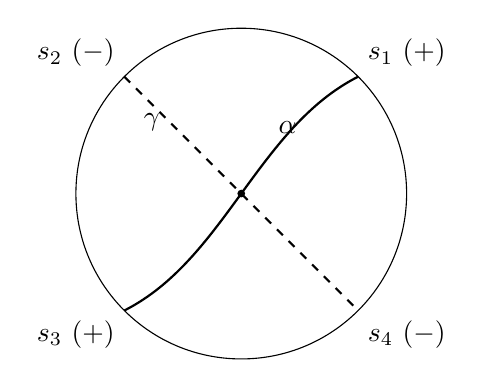
\begin{tikzpicture}[scale=1.4]
 \draw (0,0) circle (1.5);
 \draw[thick] (45:1.5) .. controls (0.15,0.6) and (-0.15,-0.6) .. (225:1.5);
 \draw[dashed,thick] (135:1.5) -- (315:1.5);
 \fill (0,0) circle (0.035);
 \node[above right] at (45:1.5) {$s_1\ (+)$};
 \node[above left] at (135:1.5) {$s_2\ (-)$};
 \node[below left] at (225:1.5) {$s_3\ (+)$};
 \node[below right] at (315:1.5) {$s_4\ (-)$};
 \node[right] at (0.25,0.6) {$\alpha$};
 \node[left] at (-0.65,0.65) {$\gamma$};
\end{tikzpicture}
\caption{Schematic of the forbidden alternating-sign configuration.
The positive crosscut $\alpha$ joins $s_1$ to $s_3$. The putative
negative path $\gamma$ joins the other two boundary points and must
intersect $\alpha$ by \cref{fact:crosscut}. The particular shapes drawn
are illustrative; the theorem applies to the paths constructed in
\cref{lem:nodal-components}.}\label{fig:alternating-signs}
\end{figure}

The following bound is due to Nadirashvili
\cite[Theorem 3, p.~227]{Nadirashvili}; see also
\cite[Proposition 2.5]{BanuelosBurdzy}. We give the boundary-sign proof.

\begin{proposition}\label[proposition]{prop:multiplicity}
The real eigenspace $V$ has dimension at most two.
\end{proposition}
\begin{proof}
Suppose $\dim_{\mathbb R}V\ge3$. Consider the real linear map
\[
 T:V\to\mathbb R^2,\qquad
 T(v)=\left(\int_{S^1}\beta h_v\cos\theta\,ds,
             \int_{S^1}\beta h_v\sin\theta\,ds\right),
 \qquad s=e^{i\theta}.
\]
Its rank is at most two, so its kernel contains a nonzero $v$.
By \cref{lem:boundary-weight}, the trace $h=h_v$ is nonzero, takes
both signs, and satisfies
\begin{equation}\label{eq:three-moments}
 \int_{S^1}\beta h\,ds
 =\int_{S^1}\beta h\cos\theta\,ds
 =\int_{S^1}\beta h\sin\theta\,ds=0.
\end{equation}

Choose a strictly negative point $e^{i\theta_0}$ and cut the circle
there, parametrizing the other points by
$\theta\in(\theta_0,\theta_0+2\pi)$. Write
$H(\theta)=h(e^{i\theta})$, $B(\theta)=\beta(e^{i\theta})$, and
\[
 A=\{\theta\in(\theta_0,\theta_0+2\pi):H(\theta)>0\},
 \qquad a=\inf A,\quad b=\sup A.
\]
The set $A$ is nonempty and open. Continuity and strict negativity at
the cut give negative neighbourhoods at both ends of the angle
interval. Therefore
\[
 \theta_0<a<b<\theta_0+2\pi.
\]
Continuity gives $H(a)=H(b)=0$, and the definitions give $H\le0$
outside $[a,b]$. There is no negative value at any
$\theta\in(a,b)$: the definitions of infimum and supremum provide
positive angles $\theta_-<\theta<\theta_+$ in $A$. The cut point,
$e^{i\theta_-}$, $e^{i\theta}$ and $e^{i\theta_+}$ would then have
strictly alternating signs in cyclic order, contradicting
\cref{lem:nodal-components}. Hence $H\ge0$ on $[a,b]$.

Set $c=(a+b)/2$ and $d=(b-a)/2\in(0,\pi)$, and define the
$2\pi$-periodic function
\[
 F(\theta)=\cos(\theta-c)-\cos d.
\]
On the circle, $F>0$ precisely on the arc represented by $(a,b)$,
$F=0$ at its endpoints, and $F<0$ on the complementary open arc.
This follows from strict decrease of cosine on $[0,\pi]$, using
angular distance from $c$ in $[0,\pi]$. Thus $FH\ge0$ everywhere,
and $FH>0$ on the nonempty open set $A$. Since $B>0$,
\[
 \int_{\theta_0}^{\theta_0+2\pi} B(\theta)F(\theta)H(\theta)\,d\theta>0.
\]
On the other hand,
\[
 F(\theta)=\cos c\cos\theta+\sin c\sin\theta-\cos d,
\]
so \cref{eq:three-moments}, together with $ds=d\theta$, makes this
same integral zero. The contradiction proves $\dim_{\mathbb R}V\le2$.
\end{proof}

% Included by main.tex; the preamble and references are shared.
\section{A variational principle for tangent vector fields}\label{sec:vector-fields}

For $X\in H^1(\Omega;\mathbb R^2)$, \emph{tangent trace} means
$\operatorname{Tr}X\cdot\nu=0$ almost everywhere on $\partial\Omega$;
see \cite[Theorem 1.1, p.~2]{Rohleder} for this boundary condition.
For any $X\in H^1(\Omega;\mathbb R^2)$ define
\[
 Q(X)=\int_\Omega\bigl(|\operatorname{div}X|^2
                         +|\operatorname{curl}X|^2\bigr),
 \qquad \operatorname{curl}X=\partial_1X_2-\partial_2X_1.
\]
The following is the divergence--curl form of Rohleder's vector
variational principle \cite[Theorem 1.1]{Rohleder}; see also \cite{Roh24}.
We give its derivation,
including the equality case.

\begin{proposition}\label[proposition]{prop:vector-variational}
For every $X\in H^1(\Omega;\mathbb R^2)$ with tangent trace,
\begin{equation}\label{eq:vector-inequality}
 Q(X)\ge\lambda_N\|X\|_2^2.
\end{equation}
Equality holds if and only if $X=\nabla v$ for some $v\in V$.
\end{proposition}
\begin{proof}
We use the Sobolev integration-by-parts identity
\begin{equation}\label{eq:sobolev-ibp}
 \int_\Omega Y\cdot\nabla u
 =-\int_\Omega u\,\operatorname{div}Y
   +\int_{\partial\Omega}\operatorname{Tr}u\,
        (\operatorname{Tr}Y\cdot\nu)\,d\sigma,
\end{equation}
valid for $u\in H^1(\Omega;\mathbb R)$ and
$Y\in H^1(\Omega;\mathbb R^2)$. It follows from the classical divergence
theorem by smooth approximation in $H^1$ and continuity of the trace
into $L^2(\partial\Omega)$; see \cite[Theorem 1.46, Theorem 3.44,
and Section 3.11]{Hunter}. The boundary product is integrable by
Cauchy--Schwarz.

First solve
\begin{equation}\label{eq:potentials}
 \begin{aligned}
 \Delta v&=\operatorname{div}X,\qquad
 \partial_\nu v=0,\qquad \int_\Omega v=0,\\
 \Delta j&=\operatorname{curl}X,\qquad \operatorname{Tr}j=0.
 \end{aligned}
\end{equation}
For the Neumann problem, the required compatibility condition is
\[
 \int_\Omega\operatorname{div}X
 =\int_{\partial\Omega}\operatorname{Tr}X\cdot\nu\,d\sigma=0.
\]
Here we applied \cref{eq:sobolev-ibp} with $u=1$ and $Y=X$.
On the closed mean-zero subspace
\[
 H=\left\{w\in H^1(\Omega;\mathbb R):\int_\Omega w=0\right\},
\]
the form $a(v,w)=\int_\Omega\nabla v\cdot\nabla w$ is continuous and
coercive by the mean-zero Poincar\'e inequality. Since
$\operatorname{div}X\in L^2(\Omega)$, Lax--Milgram
\cite[Theorem 4.20, p.~103]{Hunter} gives a unique $v\in H$ such that
\[
 \int_\Omega\nabla v\cdot\nabla w
 =-\int_\Omega(\operatorname{div}X)w\qquad(w\in H).
\]
Compatibility extends this identity to all $w\in H^1(\Omega;\mathbb R)$
by subtracting their means. It is the weak formulation of the Neumann
problem in \cref{eq:potentials}.
Similarly, the Dirichlet Poincar\'e inequality makes $a$ coercive on
$H_0^1(\Omega;\mathbb R)$, so Lax--Milgram gives a unique
$j\in H_0^1(\Omega;\mathbb R)$ satisfying
\[
 \int_\Omega\nabla j\cdot\nabla w
 =-\int_\Omega(\operatorname{curl}X)w
 \qquad(w\in H_0^1(\Omega;\mathbb R)).
\]
No compatibility condition is needed for this Dirichlet problem.
Boundary regularity gives $v,j\in H^2(\Omega)$; see
\cite[Chapter III, Theorems 6.1 and 6.4]{Showalter}.

Put $\nabla^\perp j=(-\partial_2j,\partial_1j)$.
Tangential differentiation commutes with taking the trace for $H^2$
functions on a smooth domain; this follows by smooth approximation and
continuity of the trace maps. Thus the zero trace of $j$ implies that
$\nabla^\perp j$ has tangent trace. Consequently
\[
 Z=X-\nabla v-\nabla^\perp j
\]
belongs to $H^1(\Omega;\mathbb R^2)$ and has tangent trace.
The equations in \cref{eq:potentials} give
$\operatorname{div}Z=\operatorname{curl}Z=0$. Its components are
harmonic in distributions and hence smooth in the interior by Weyl's
lemma. Simple connectivity therefore gives a smooth real interior
potential $r$ with $Z=\nabla r$.

For $M>0$, define $r_M=\max\{-M,\min\{r,M\}\}$, and write
$s^+=\max\{s,0\}$.
The weak derivative formulas for positive parts
\cite[Proposition 3.22 and the subsequent discussion, pp.~57--58]{Hunter},
applied locally to
$r_M=r-(r-M)^++(-r-M)^+$, give
\[
 r_M\in H^1_{\mathrm{loc}}(\Omega),\qquad
 \nabla r_M=\mathbf1_{\{|r|<M\}}Z\quad\text{almost everywhere}.
\]
Since $|r_M|\le M$, $\Omega$ is bounded, and $Z\in L^2(\Omega)$,
it follows that $r_M\in H^1(\Omega)$.

Fix a ball $B$ with $\overline B\subset\Omega$, and write $u_B$ and
$u_\Omega$ for the averages over $B$ and $\Omega$. The usual mean-zero
Poincar\'e inequality gives, for $u\in H^1(\Omega)$,
\[
 \begin{aligned}
 |u_B-u_\Omega|
 &\le |B|^{-1/2}\|u-u_\Omega\|_2,\\
 \|u-u_B\|_2
 &\le\left(1+\sqrt{\frac{|\Omega|}{|B|}}\right)
       \|u-u_\Omega\|_2\\
 &\le C_{\Omega,B}\|\nabla u\|_2.
 \end{aligned}
\]
Applying this to $r_M$ and using $|r_M|\le|r|$ on $B$ yields
\[
 \|r_M\|_2
 \le C_{\Omega,B}\|Z\|_2
       +|\Omega|^{1/2}|(r_M)_B|
 \le C_{\Omega,B}\|Z\|_2
       +|\Omega|^{1/2}\sup_B|r|.
\]
The bound is independent of $M$. Since $r_M\to r$ pointwise, Fatou's
lemma gives $r\in L^2(\Omega)$. Moreover, for every
$\phi\in C_c^\infty(\Omega)$,
\[
 \int_\Omega r\,\partial_i\phi=-\int_\Omega Z_i\phi
 \qquad(i=1,2),
\]
by the interior identity $\nabla r=Z$. Thus the global weak gradient of
$r$ is $Z$, and $r\in H^1(\Omega)$. This establishes its global
integrability using only the interior potential and $Z\in L^2$.
Applying \cref{eq:sobolev-ibp} with $u=r$ and $Y=Z$ now gives
\[
 \int_\Omega|\nabla r|^2
 =\int_\Omega Z\cdot\nabla r
 =-\int_\Omega r\,\operatorname{div}Z
   +\int_{\partial\Omega}\operatorname{Tr}r\,
        (\operatorname{Tr}Z\cdot\nu)\,d\sigma=0.
\]
Hence $Z=0$, and
\begin{equation}\label{eq:decomposition}
 X=\nabla v+\nabla^\perp j.
\end{equation}
The summands are orthogonal in $L^2$, since
\[
 \int_\Omega\nabla v\cdot\nabla^\perp j
 =-\int_\Omega v\,\operatorname{div}(\nabla^\perp j)
   +\int_{\partial\Omega}\operatorname{Tr}v\,
       (\operatorname{Tr}\nabla^\perp j\cdot\nu)\,d\sigma=0.
\]
Consequently
\[
 \|X\|_2^2=\|\nabla v\|_2^2+\|\nabla j\|_2^2,
 \qquad Q(X)=\|\Delta v\|_2^2+\|\Delta j\|_2^2.
\]

Integration by parts, Cauchy--Schwarz, and the two Poincar\'e inequalities
give
\[
 \begin{aligned}
 \|\nabla v\|_2^2
 &=-\int_\Omega v\,\Delta v
 \le\|v\|_2\|\Delta v\|_2\\
 &\le\lambda_N^{-1/2}\|\nabla v\|_2\|\Delta v\|_2,\\
 \|\nabla j\|_2^2
 &=-\int_\Omega j\,\Delta j
 \le\|j\|_2\|\Delta j\|_2\\
 &\le\lambda_D^{-1/2}\|\nabla j\|_2\|\Delta j\|_2.
 \end{aligned}
\]
The boundary terms vanish because $\partial_\nu v=0$ and
$\operatorname{Tr}j=0$, respectively. The last inequalities use the
zero mean of $v$ and the zero trace of $j$. Dividing by the gradient
norms when nonzero, with the zero cases immediate, gives
\[
 \|\Delta v\|_2^2\ge\lambda_N\|\nabla v\|_2^2,
 \qquad
 \|\Delta j\|_2^2\ge\lambda_D\|\nabla j\|_2^2.
\]
It follows that
\begin{equation}\label{eq:vector-refined}
 \begin{aligned}
 Q(X)&\ge\lambda_N\|\nabla v\|_2^2
              +\lambda_D\|\nabla j\|_2^2\\
 &=\lambda_N\|X\|_2^2
              +(\lambda_D-\lambda_N)\|\nabla j\|_2^2.
 \end{aligned}
\end{equation}
This proves \cref{eq:vector-inequality}.

Suppose equality holds in \cref{eq:vector-inequality}.
Since $\lambda_D>\lambda_N$, \cref{eq:vector-refined} forces
$\nabla j=0$, and the zero trace gives $j=0$. Thus $X=\nabla v$ and
$\|\Delta v\|_2^2=\lambda_N\|\nabla v\|_2^2$.
If $\nabla v\ne0$, the preceding chain becomes
\[
 \begin{aligned}
 \|\nabla v\|_2^2
 &\le\|v\|_2\|\Delta v\|_2\\
 &\le\lambda_N^{-1/2}\|\nabla v\|_2\|\Delta v\|_2
 =\|\nabla v\|_2^2.
 \end{aligned}
\]
Both inequalities are equalities, so
$\|\nabla v\|_2^2=\lambda_N\|v\|_2^2$.
The equality characterization of the mean-zero Neumann variational
inequality (Fact~2.2 of the spectral and planar preliminaries) gives
\cref{eq:V-weak}, hence $v\in V$.
If $\nabla v=0$, its zero mean gives $v=0\in V$.

Conversely, if $v\in V$, then $X=\nabla v$ belongs to
$H^1(\Omega;\mathbb R^2)$ and has tangent trace because
$\partial_\nu v=0$. Also $\operatorname{curl}X=0$ and
$\operatorname{div}X=\Delta v=-\lambda_Nv$, so
\[
 Q(X)=\lambda_N^2\|v\|_2^2
      =\lambda_N\|\nabla v\|_2^2
      =\lambda_N\|X\|_2^2,
\]
where the middle equality follows by testing \cref{eq:V-weak} with $v$.
\end{proof}

For a differential-form interpretation of the divergence--curl energy,
see \cite[Section 5.1]{FGM26}.

We next record the boundary identity in fixed Cartesian coordinates.
Let $\tau=(-\nu_2,\nu_1)$ be the counterclockwise unit tangent, and set
\[
 \kappa=\det(\tau,\partial_\tau\tau).
\]
Thus $\kappa$ is positive on a convex circle. Here
$|\nabla X|^2=\sum_{i,j=1}^2(\partial_iX_j)^2$.

\begin{lemma}\label[lemma]{lem:curvature-identity}
For every $X\in H^1(\Omega;\mathbb R^2)$ with tangent trace,
\begin{equation}\label{eq:curvature-identity}
 Q(X)=\int_\Omega|\nabla X|^2
       +\int_{\partial\Omega}\kappa|\operatorname{Tr}X|^2\,d\sigma.
\end{equation}
\end{lemma}
\begin{proof}
First suppose $X\in C^\infty(\overline\Omega;\mathbb R^2)$, without
imposing tangency. Expanding the bulk integrands gives
\[
 \begin{aligned}
 &|\operatorname{div}X|^2+|\operatorname{curl}X|^2-|\nabla X|^2\\
 &\quad=(\partial_1X_1+\partial_2X_2)^2
        +(\partial_1X_2-\partial_2X_1)^2\\
 &\qquad\quad-\sum_{i,j=1}^2(\partial_iX_j)^2\\
 &\quad=2\bigl(\partial_1X_1\,\partial_2X_2
              -\partial_1X_2\,\partial_2X_1\bigr)
        =2\det\nabla X.
 \end{aligned}
\]
Put
\[
 F=\bigl(X_1\partial_2X_2-X_2\partial_2X_1,\,
         X_2\partial_1X_1-X_1\partial_1X_2\bigr).
\]
The mixed second derivatives cancel, so
$\operatorname{div}F=2\det\nabla X$. On the boundary,
\[
 F\cdot\nu=X_1\partial_\tau X_2-X_2\partial_\tau X_1.
\]
The divergence theorem therefore gives
\begin{equation}\label{eq:smooth-boundary-pairing}
 Q(X)-\int_\Omega|\nabla X|^2
 =\int_{\partial\Omega}
   \bigl(X_1\partial_\tau X_2-X_2\partial_\tau X_1\bigr)\,d\sigma.
\end{equation}

For $h=(h_1,h_2)\in H^{1/2}(\partial\Omega;\mathbb R^2)$, define
\[
 B(h)=\langle\partial_\tau h_2,h_1\rangle
       -\langle\partial_\tau h_1,h_2\rangle,
\]
where the brackets denote the real $H^{-1/2}$--$H^{1/2}$ duality
pairing, agreeing with the boundary integral for smooth functions.
Tangential differentiation is bounded from $H^{1/2}(\partial\Omega)$
to $H^{-1/2}(\partial\Omega)$, so $B$ is continuous on $H^{1/2}$.
Choose $X_n\in C^\infty(\overline\Omega;\mathbb R^2)$ converging to
$X\in H^1(\Omega;\mathbb R^2)$ in $H^1$. Their traces converge to
$h=\operatorname{Tr}X$ in $H^{1/2}$, hence
$B(\operatorname{Tr}X_n)\to B(h)$. The bulk integrals also converge,
since the first derivatives converge in $L^2$. Passing to the limit in
\cref{eq:smooth-boundary-pairing} gives
\begin{equation}\label{eq:sobolev-boundary-pairing}
 Q(X)-\int_\Omega|\nabla X|^2=B(h).
\end{equation}
The approximating fields need not have tangent trace.

Now suppose $h$ is tangent, and put $a=h\cdot\tau$, so $h=a\tau$.
Multiplication by the smooth components of $\tau$ preserves $H^{1/2}$,
and hence $a\in H^{1/2}(\partial\Omega;\mathbb R)$.
First take $a$ smooth. The product rule gives
\[
 \begin{aligned}
 B(a\tau)
 &=\int_{\partial\Omega}
   \bigl[a\tau_1\partial_\tau(a\tau_2)
         -a\tau_2\partial_\tau(a\tau_1)\bigr]\,d\sigma\\
 &=\int_{\partial\Omega}
       a^2\det(\tau,\partial_\tau\tau)\,d\sigma
 =\int_{\partial\Omega}\kappa a^2\,d\sigma,
 \end{aligned}
\]
because the terms containing $a\,\partial_\tau a$ cancel.
For general $a\in H^{1/2}$, choose smooth $a_n\to a$ in $H^{1/2}$.
Then $a_n\tau\to a\tau$ in $H^{1/2}$, so continuity of $B$ gives
$B(a_n\tau)\to B(a\tau)$. Also $a_n\to a$ in $L^2$, and
\[
 \|a_n^2-a^2\|_{L^1(\partial\Omega)}
 \le\|a_n-a\|_{L^2(\partial\Omega)}
      \bigl(\|a_n\|_{L^2(\partial\Omega)}
            +\|a\|_{L^2(\partial\Omega)}\bigr)\to0.
\]
Since $\kappa$ is bounded, we may pass to the limit to obtain
$B(a\tau)=\int_{\partial\Omega}\kappa a^2\,d\sigma$.
Finally $|h|^2=a^2$, and \cref{eq:sobolev-boundary-pairing} proves
\cref{eq:curvature-identity}.
\end{proof}

% Included by main.tex; the preamble and references are shared.
\section{Boundary kernels and the multiplier identity}\label{sec:boundary-kernels}

\subsection{A subcritical disk potential}

Let $\Omega\subset\mathbb R^2$ be a nonempty bounded simply connected
open set with smooth boundary, and fix the smooth conformal
diffeomorphism $\Phi:\overline{\mathbb D}\to\overline\Omega$ constructed
in \cref{lem:conformal}. Here
$\mathbb D=\{z\in\mathbb C:|z|<1\}$ and $S^1=\partial\mathbb D$.
Write $\lambda_D$ and $\lambda_N$ for the first Dirichlet and first
positive Neumann eigenvalues of $\Omega$, respectively. Define
\begin{equation}\label{eq:conformal-measure}
 dq(x)=\lambda_N|\Phi'(x)|^2\,dx.
\end{equation}
Its density is bounded and positive. We use real scalar functions and
write $\langle f,g\rangle_q=\int_{\mathbb D}fg\,dq$ and
$\|f\|_q^2=\langle f,f\rangle_q$.

For $\eta\in H_0^1(\mathbb D)$, put $u=\eta\circ\Phi^{-1}$.
The smooth diffeomorphism preserves zero trace, so
$u\in H_0^1(\Omega)$. Conformality gives
$D\Phi=|\Phi'|R$, where $R$ is a rotation, and
$\det D\Phi=|\Phi'|^2$. Thus the chain rule and change of variables give
\[
 \int_\Omega|\nabla u|^2\,dy
 =\int_{\mathbb D}|\nabla\eta|^2\,dx.
\]
These identities hold first for smooth functions and then by density
in $H_0^1$. The Dirichlet inequality on $\Omega$ therefore gives
\[
 \|\eta\|_q^2
 =\lambda_N\int_\Omega u^2\,dy
 \le\frac{\lambda_N}{\lambda_D}\int_\Omega|\nabla u|^2\,dy
 =\frac{\lambda_N}{\lambda_D}
       \int_{\mathbb D}|\nabla\eta|^2\,dx.
\]
The spectral comparison \cref{lem:spectral-gap} gives
$\lambda_N<\lambda_D$. Hence
\begin{equation}\label{eq:weighted-dirichlet}
 \|\eta\|_q^2\le d\int_{\mathbb D}|\nabla\eta|^2\,dx
 \qquad(\eta\in H_0^1(\mathbb D)),
 \qquad d=\frac{\lambda_N}{\lambda_D}<1.
\end{equation}

For the scalar kernel construction, we allow any measure $dq=a\,dx$
with bounded nonnegative density satisfying
\cref{eq:weighted-dirichlet} for some fixed $0<d<1$.
The conformal measure \cref{eq:conformal-measure} is one such measure;
the zero measure is also allowed.

The Dirichlet Green function of the disk is
\begin{equation}\label{eq:disk-green}
 G(x,y)=\frac1{2\pi}\log\left|
                  \frac{1-\overline{x}y}{x-y}\right|
 =\frac1{4\pi}\log\left(
       1+\frac{(1-|x|^2)(1-|y|^2)}{|x-y|^2}\right),
 \qquad x\ne y.
\end{equation}
It is nonnegative and symmetric, vanishes when either variable lies
on $S^1$, and has logarithmic singularity
$-(2\pi)^{-1}\log|x-y|$. Its diagonal value is set to $+\infty$;
the diagonal has measure zero in all integrals below.
For fixed $x\in\mathbb D$, it is harmonic in $y$ away from $x$:
both logarithms in the first formula are logarithms of moduli of
nonvanishing holomorphic functions there.

\begin{lemma}\label[lemma]{lem:green-operator}
The operator
\[
 Tf(x)=\int_{\mathbb D}G(x,y)f(y)\,dq(y)
\]
is bounded and self-adjoint on $L^2(q)$, with $\|T\|\le d<1$.
For each $f\in L^2(q)$, the displayed integral is the continuous
interior representative of the weak Dirichlet solution of
$-\Delta\psi=af$.
For every measure $0\le\rho\le q$, the operator
\[
 T_\rho f(x)=\int_{\mathbb D}G(x,y)f(y)\,d\rho(y)
\]
has the same properties on $L^2(\rho)$, with $\|T_\rho\|\le d$.
\end{lemma}
\begin{proof}
We first justify the Green representation for a source
$b\in L^2(\mathbb D;dx)$. The Poincar\'e inequality and Lax--Milgram
\cite[Theorem 4.20, p.~103]{Hunter}
give a unique $u\in H_0^1(\mathbb D)$ satisfying
\begin{equation}\label{eq:weak-poisson}
 \int_{\mathbb D}\nabla u\cdot\nabla\eta\,dx
 =\int_{\mathbb D}b\eta\,dx
 \qquad(\eta\in H_0^1(\mathbb D)).
\end{equation}
If $b\in C_c^\infty(\mathbb D)$, this solution is smooth up to the
boundary. Apply Green's second identity to $u$ and $G(x,\cdot)$ on
$\mathbb D\setminus\overline{B_\varepsilon(x)}$.
The outer boundary term is zero. On the inner circle, whose outward
normal points towards $x$,
\[
 G(x,y)=-\frac1{2\pi}\log\varepsilon+O(1),
 \qquad \partial_\nu G(x,y)=\frac1{2\pi\varepsilon}+O(1).
\]
Consequently the integral of
$G\partial_\nu u-u\partial_\nu G$ tends to $-u(x)$.
Since $\Delta_yG(x,y)=0$ away from $x$ and $\Delta u=-b$,
letting $\varepsilon\downarrow0$ gives
\begin{equation}\label{eq:green-representation}
 u(x)=\int_{\mathbb D}G(x,y)b(y)\,dy.
\end{equation}

For general $b\in L^2(dx)$, choose $b_n\in C_c^\infty(\mathbb D)$
converging to $b$ in $L^2$, and let $u_n$ be their weak solutions.
Testing the difference equation and using Poincar\'e gives
\[
 \|\nabla(u_n-u)\|_2^2
 \le C\|b_n-b\|_2\|\nabla(u_n-u)\|_2.
\]
Thus $u_n\to u$ in $H_0^1$, and a subsequence converges almost
everywhere. For each fixed $x\in\mathbb D$, the logarithmic pole is
square integrable, so $G(x,\cdot)\in L^2(dx)$ and
\[
 \left|\int_{\mathbb D}G(x,y)(b_n-b)(y)\,dy\right|
 \le\|G(x,\cdot)\|_2\|b_n-b\|_2\longrightarrow0.
\]
Passing to the limit in \cref{eq:green-representation} proves that
its right-hand side equals $u$ almost everywhere.

To prove continuity of this representative, fix $K\Subset\mathbb D$
and $r<1$ with $|x|\le r$ on $K$. For $x,x_0\in K$,
\[
 \left|\log|1-\overline{x}y|
           -\log|1-\overline{x_0}y|\right|
 \le\frac{|x-x_0|}{1-r}\qquad(y\in\mathbb D).
\]
For the singular part choose $\chi\in C_c^\infty(\mathbb R^2)$
equal to one on $\{|z|\le2\}$ and set $F(z)=\chi(z)\log|z|$.
Then $F\in L^2(\mathbb R^2)$, since
$\int_0^1 t|\log t|^2\,dt<\infty$, and
\[
 \|\log|x-\cdot|-\log|x_0-\cdot|\|_{L^2(\mathbb D)}
 \le\|F(x-\cdot)-F(x_0-\cdot)\|_{L^2(\mathbb R^2)}
 \longrightarrow0.
\]
Here continuity of translations in $L^2$ follows by approximation
by smooth compactly supported functions: translation preserves the
$L^2$ norm, and the translated approximants converge in $L^2$.
Together with \cref{eq:disk-green}, these estimates give
$\|G(x,\cdot)-G(x_0,\cdot)\|_2\to0$. Hence
\[
 \left|\int_{\mathbb D}(G(x,y)-G(x_0,y))b(y)\,dy\right|
 \le\|G(x,\cdot)-G(x_0,\cdot)\|_2\|b\|_2\longrightarrow0.
\]
This proves the asserted interior continuity.

Now let $f\in L^2(q)$. The source $af$ belongs to $L^2(dx)$ because
\[
 \int_{\mathbb D}|af|^2\,dx
 \le\|a\|_\infty\int_{\mathbb D}|f|^2\,dq.
\]
Changing $f$ on a $q$-null set does not change $af$ almost everywhere
with respect to $dx$, so the integral defines a linear map on $L^2(q)$.
The representation just proved identifies $\psi=Tf$ with the weak
solution for $b=af$. Taking $\eta=\psi$ in \cref{eq:weak-poisson}
gives
\[
 \int_{\mathbb D}|\nabla\psi|^2\,dx
 =\int_{\mathbb D}af\psi\,dx=\langle\psi,f\rangle_q.
\]
Thus \cref{eq:weighted-dirichlet} and Cauchy--Schwarz imply
\[
 \|\psi\|_q^2
 \le d\int_{\mathbb D}|\nabla\psi|^2\,dx
 =d\langle\psi,f\rangle_q
 \le d\|\psi\|_q\|f\|_q.
\]
Dividing when $\|\psi\|_q>0$, with the zero case immediate, proves
$\|T\|\le d$.

For self-adjointness, \cref{eq:disk-green} gives
$G(x,y)=G(y,x)$ and
\[
 0\le G(x,y)\le\frac1{2\pi}\log\frac2{|x-y|}.
\]
The square of the upper bound is integrable on
$\mathbb D\times\mathbb D$; boundedness of $a$ therefore gives
$G\in L^2(q\times q)$. For $f,g\in L^2(q)$, Cauchy--Schwarz on the
product space gives
\[
 \iint G(x,y)|f(y)g(x)|\,dq(y)\,dq(x)
 \le\|G\|_{L^2(q\times q)}\|f\|_q\|g\|_q<\infty.
\]
Fubini and symmetry now yield
\[
 \langle Tf,g\rangle_q
 =\iint G(x,y)f(y)g(x)\,dq(y)\,dq(x)
 =\langle f,Tg\rangle_q.
\]
Since $T$ is bounded and defined on all of $L^2(q)$, it is self-adjoint.

Finally, $0\le\rho\le q$ means $\rho(E)\le q(E)$ for every
measurable set $E$. It follows that $d\rho=c\,dx$ with
$0\le c\le a$ almost everywhere, so $c$ is bounded. Moreover,
\[
 \|\eta\|_{L^2(\rho)}^2
 \le\|\eta\|_q^2
 \le d\int_{\mathbb D}|\nabla\eta|^2\,dx
 \qquad(\eta\in H_0^1(\mathbb D)).
\]
This is the estimate needed to bound the solution operator on
$L^2(\rho)$. Indeed, for $f\in L^2(\rho)$ the source $cf$ lies in
$L^2(dx)$, and its weak solution $\psi=T_\rho f$ satisfies
\[
 \|\psi\|_{L^2(\rho)}^2
 \le d\int_{\mathbb D}|\nabla\psi|^2\,dx
 =d\int_{\mathbb D}f\psi\,d\rho
 \le d\|f\|_{L^2(\rho)}\|\psi\|_{L^2(\rho)}.
\]
Thus $\|T_\rho\|\le d$. The same Green representation proves
interior continuity, and the same Fubini argument with $c$ in place
of $a$ proves self-adjointness.
\end{proof}

For Lipschitz boundary data $h:S^1\to\mathbb R$, define the Poisson
extension
\begin{equation}\label{eq:poisson-extension}
 Ah(x)=\int_{S^1}P_s(x)h(s)\,ds,
 \qquad P_s(x)=\frac{1-|x|^2}{2\pi|s-x|^2},
\end{equation}
where $ds$ is arclength on the unit circle. To justify its Sobolev
regularity, write
\[
 h(e^{i\theta})=\sum_{n\in\mathbb Z}h_ne^{in\theta},
 \qquad
 Ah(re^{i\theta})=\sum_{n\in\mathbb Z}h_nr^{|n|}e^{in\theta}.
\]
Lipschitz regularity gives $h\in H^1(S^1)$, so
$\sum_n(1+n^2)|h_n|^2<\infty$. Parseval's identity and integration
in polar coordinates give
\[
 \|Ah\|_{L^2(\mathbb D)}^2
 =\pi\sum_{n\in\mathbb Z}\frac{|h_n|^2}{|n|+1},
 \qquad
 \|\nabla Ah\|_{L^2(\mathbb D)}^2
 =2\pi\sum_{n\in\mathbb Z}|n|\,|h_n|^2.
\]
These identities hold first for finite Fourier sums; their harmonic
extensions converge in $H^1(\mathbb D)$ by the displayed bounds.
Their boundary values converge to $h$ in $H^1(S^1)$, so continuity
of the trace shows that $\operatorname{Tr}Ah=h$. Harmonicity also
passes to the limit, giving
\[
 \int_{\mathbb D}\nabla Ah\cdot\nabla\eta\,dx=0
 \qquad(\eta\in H_0^1(\mathbb D)).
\]

We seek $W_h\in H^1(\mathbb D)$ with trace $h$ satisfying
\begin{equation}\label{eq:weak-potential-solution}
 \int_{\mathbb D}\nabla W_h\cdot\nabla\eta\,dx
 =\int_{\mathbb D}aW_h\eta\,dx
 \qquad(\eta\in H_0^1(\mathbb D)).
\end{equation}
This is the weak meaning of $-\Delta W_h\,dx=W_h\,dq$.
Existence and uniqueness follow from Lax--Milgram
\cite[Theorem 4.20, p.~103]{Hunter} after writing
$W_h=Ah+c$, $c\in H_0^1(\mathbb D)$. Indeed, the continuous form
\[
 B(u,\eta)=\int_{\mathbb D}\nabla u\cdot\nabla\eta\,dx
           -\int_{\mathbb D}au\eta\,dx
\]
satisfies
$B(c,c)\ge(1-d)\|\nabla c\|_2^2$ by
\cref{eq:weighted-dirichlet}, and the correction equation is
$B(c,\eta)=\int_{\mathbb D}aAh\,\eta\,dx$.

The solution has the explicit representation
\begin{equation}\label{eq:potential-extension}
 W_h=Ah+T(I-T)^{-1}Ah.
\end{equation}
To verify it, boundedness of $a$ gives $Ah\in L^2(q)$, and
\cref{lem:green-operator} gives
$(I-T)^{-1}=\sum_{n\ge0}T^n$ in operator norm on $L^2(q)$.
Put $v=(I-T)^{-1}Ah$ and $c=Tv$. Then
$c\in H_0^1(\mathbb D)$, and the weak Poisson equation gives
\[
 \int_{\mathbb D}\nabla c\cdot\nabla\eta\,dx
 =\int_{\mathbb D}av\eta\,dx
 \qquad(\eta\in H_0^1(\mathbb D)).
\]
The identity $(I-T)v=Ah$ implies $v=Ah+c=W_h$ in $L^2(q)$.
Consequently harmonicity of $Ah$ yields
\[
 \int_{\mathbb D}\nabla W_h\cdot\nabla\eta\,dx
 =\int_{\mathbb D}\nabla c\cdot\nabla\eta\,dx
 =\int_{\mathbb D}aW_h\eta\,dx.
\]
Also $\operatorname{Tr}W_h=h$, since $c$ has zero trace.
For a direct uniqueness check, the difference $z$ of two solutions
with this trace lies in $H_0^1(\mathbb D)$. Testing its equation by
$z$ and using \cref{eq:weighted-dirichlet} gives
\[
 \|\nabla z\|_2^2=\|z\|_q^2\le d\|\nabla z\|_2^2.
\]
Since $d<1$, $\nabla z=0$, and Poincar\'e gives $z=0$.
For vector boundary data all constructions and equations are
understood componentwise.

\subsection{Positive kernels and their estimates}

For $s\in S^1$, define $U_{0,s}=P_s$ and recursively set
\[
 U_{n+1,s}(x)=\int_{\mathbb D}G(x,y)U_{n,s}(y)\,dq(y).
\]
The nonnegative integrands define measurable functions with values in
$[0,\infty]$. We write $T^nP_s=U_{n,s}$; this definition does not
require $P_s\in L^2(q)$. Finiteness is established below.
For $p\in\mathbb D$ and distinct $s,t\in S^1$, define
\begin{align}
 K(p,s)&=P_s(p)+\sum_{n\ge1}(T^nP_s)(p),
                    \label{eq:solution-kernel}\\
 R(s,t)&=\sum_{n\ge0}\int_{\mathbb D}P_sT^nP_t\,dq,
                    \label{eq:interaction-kernel}\\
 N(s,t)&=N_0(s,t)+R(s,t),
 \qquad N_0(s,t)=\frac1{\pi|s-t|^2}.
                    \label{eq:boundary-kernel}
\end{align}
For integrations we also define $R$ on the diagonal by the same
nonnegative series, allowing the value $+\infty$.

\begin{lemma}\label[lemma]{lem:kernel-estimates}
The kernels in \cref{eq:solution-kernel,eq:interaction-kernel,eq:boundary-kernel}
are finite at the stated points. For fixed $p\in\mathbb D$,
$K(p,\cdot)$ is positive and bounded. The kernel $R$ is symmetric,
nonnegative, and integrable on $S^1\times S^1$, with
\begin{equation}\label{eq:interaction-mass}
 \iint_{S^1\times S^1}R(s,t)\,ds\,dt
 \le\frac{q(\mathbb D)}{1-d}.
\end{equation}
For Lipschitz scalar or vector boundary data $h,k$,
\begin{align}
 W_h(p)&=\int_{S^1}K(p,s)h(s)\,ds,
                         \label{eq:solution-representation}\\
 \langle Ah,(I-T)^{-1}Ak\rangle_q
 &=\iint_{S^1\times S^1}R(s,t)h(s)\cdot k(t)\,ds\,dt.
                         \label{eq:interaction-representation}
\end{align}
For scalar data the dot denotes multiplication; for vector data the
inner product on the left is the sum of the component inner products.
\end{lemma}
\begin{proof}
Constants below are independent of interior and boundary points,
unless stated otherwise. The explicit formulas give
\begin{equation}\label{eq:elementary-kernel-bounds}
 P_s(y)\le\frac1{\pi|y-s|},
 \qquad 0\le G(x,y)\le\frac1{2\pi}\log\frac2{|x-y|}.
\end{equation}
For the first bound use $1-|y|^2\le2|y-s|$; for the second use
$|1-\overline{x}y|\le2$. Translating the centres and integrating
over a disk of radius two gives
\[
 \sup_{s\in S^1}\|P_s\|_{L^{3/2}(dx)}<\infty,
 \qquad
 \sup_{x\in\mathbb D}\|G(x,\cdot)\|_{L^3(dx)}<\infty,
\]
since $\int_0^2 r^{-3/2}r\,dr$ and
$\int_0^2(\log(2/r))^3r\,dr$ are finite.

Define the Green potential $F_s=TP_s$. We use it as the starting
point for the $L^2(q)$ contraction estimate. Writing $dq=a\,dy$,
H\"older's inequality with exponents $3$ and $3/2$ gives
\begin{equation}\label{eq:first-green-bound}
 F_s(x)=\int_{\mathbb D}G(x,y)P_s(y)a(y)\,dy
 \le\|a\|_\infty\|G(x,\cdot)\|_{L^3(dx)}
                   \|P_s\|_{L^{3/2}(dx)}\le C.
\end{equation}
Thus Green integration regularises the singularity of $P_s$ at
$s$, producing a bounded function, with
$\|F_s\|_q\le Cq(\mathbb D)^{1/2}$. The recursively defined
integrals satisfy $T^nP_s=T^{n-1}F_s$ for $n\ge1$, with the
right-hand side interpreted as the $L^2(q)$ operator iterates and,
for $n\ge2$, their Green representatives.
Since $q$ has bounded density, the uniform $L^3(dx)$ bound above
also gives $\sup_p\|G(p,\cdot)\|_q<\infty$. Hence, for $n\ge2$,
\begin{equation}\label{eq:geometric-kernel-bound}
 (T^nP_s)(p)
 =\langle G(p,\cdot),T^{n-2}F_s\rangle_q
 \le\|G(p,\cdot)\|_q d^{n-2}\|F_s\|_q
 \le C d^{n-2}.
\end{equation}
Together with \cref{eq:first-green-bound}, this proves convergence
of the series for $K$. For fixed $p$, the function $P_s(p)$ is
positive and bounded as $s$ varies, so the same holds for $K(p,s)$.

For the zeroth term of $R$, fix $s\ne t$ and put
$\delta=|s-t|/3$. On $\mathbb D\cap B_\delta(s)$,
$|y-t|\ge2\delta$, and \cref{eq:elementary-kernel-bounds} gives
\[
 P_s(y)P_t(y)\le\frac1{2\pi^2\delta|y-s|}.
\]
This is integrable because
$\int_{B_\delta(s)}|y-s|^{-1}\,dy=2\pi\delta$.
The same argument applies near $t$. Outside these two disks,
$P_sP_t\le(\pi^2\delta^2)^{-1}$. Thus $P_sP_t\in L^1(dx)$,
and boundedness of $a$ gives $\int P_sP_t\,dq<\infty$.
Also \cref{eq:elementary-kernel-bounds} gives
$\sup_s\int_{\mathbb D}P_s\,dq\le C$. Therefore the explicit
bounds \cref{eq:first-green-bound,eq:geometric-kernel-bound} imply
\[
 \int_{\mathbb D}P_sTP_t\,dq\le C,
 \qquad
 \int_{\mathbb D}P_sT^nP_t\,dq\le C d^{n-2}\quad(n\ge2).
\]
This proves finiteness of $R(s,t)$, and hence of $N(s,t)$, for
distinct $s,t$.

For $n\ge1$, the $n$th term of $R$ is the nonnegative chain integral
\[
 \int_{\mathbb D^{n+1}}
 P_s(y_0)\left(\prod_{j=0}^{n-1}G(y_j,y_{j+1})\right)
 P_t(y_n)\,dq(y_0)\cdots dq(y_n).
\]
Reversing the variables and using symmetry of $G$ proves symmetry
in $s,t$; the zeroth term is also symmetric.
The Poisson kernel satisfies $\int_{S^1}P_s(y)\,ds=1$.
Tonelli's theorem, applied to the nonnegative chains and series,
therefore gives
\[
 \iint R(s,t)\,ds\,dt
 =\sum_{n\ge0}\langle1,T^n1\rangle_q
 \le\sum_{n\ge0}d^n\|1\|_q^2
 =\frac{q(\mathbb D)}{1-d}.
\]
This proves \cref{eq:interaction-mass}. Values on the diagonal
$s=t$ do not affect these integrals, since it has zero product
arclength measure.

We next prove \cref{eq:solution-representation}. The Neumann series
in \cref{eq:potential-extension} gives
\[
 W_h(p)=Ah(p)+\sum_{n\ge1}T^nAh(p).
\]
Indeed, the series for $(I-T)^{-1}Ah$ converges in $L^2(q)$,
and evaluation after applying $T$ is bounded by
$|Tf(p)|\le\|G(p,\cdot)\|_q\|f\|_q$.
For nonnegative scalar $h$, inserting \cref{eq:poisson-extension}
into the iterated integrals and applying Tonelli gives
\[
 T^nAh(p)=\int_{S^1}(T^nP_s)(p)h(s)\,ds
 \qquad(n\ge0).
\]
Summing gives \cref{eq:solution-representation}.
For signed bounded $h$, all exchanges are absolutely justified by
\[
 \int_{S^1}K(p,s)|h(s)|\,ds
 \le\|h\|_\infty\int_{S^1}K(p,s)\,ds<\infty,
\]
using boundedness of $K(p,\cdot)$.

Finally, the operator Neumann series gives
\[
 \langle Ah,(I-T)^{-1}Ak\rangle_q
 =\sum_{n\ge0}\langle Ah,T^nAk\rangle_q.
\]
For nonnegative scalar $h,k$, their Poisson representations and
Tonelli yield
\[
 \langle Ah,T^nAk\rangle_q
 =\iint h(s)k(t)
      \left(\int_{\mathbb D}P_sT^nP_t\,dq\right)\,ds\,dt.
\]
Summing proves \cref{eq:interaction-representation}. For signed
bounded data the required absolute domination follows from
\cref{eq:interaction-mass}:
\[
 \iint R(s,t)|h(s)k(t)|\,ds\,dt
 \le\|h\|_\infty\|k\|_\infty\frac{q(\mathbb D)}{1-d}<\infty.
\]
The vector formulas follow by applying the scalar formulas to each
component and summing.
\end{proof}

\subsection{The boundary energy}

We now return to the conformal measure \cref{eq:conformal-measure}.
A vector boundary function $h:S^1\to\mathbb R^2$ is called tangent
if $h(s)$ is tangent to $\partial\Omega$ at $\Phi(s)$.
Write $h=(h_1,h_2)$ in fixed Cartesian coordinates, and define
$W_h=(W_{h_1},W_{h_2})$, where each component is the scalar solution
in \cref{eq:potential-extension}. Set
\[
 X_h(y)=W_h(\Phi^{-1}(y)),\qquad y\in\Omega.
\]
Composition with the smooth diffeomorphism gives
$X_h\in H^1(\Omega;\mathbb R^2)$, and its trace satisfies
$\operatorname{Tr}X_h(\Phi(s))=h(s)$. Thus tangent data give tangent
trace on $\partial\Omega$.

As in the preceding section on tangent vector fields, write
\[
 Q(X)=\int_\Omega\bigl(|\operatorname{div}X|^2
                         +|\operatorname{curl}X|^2\bigr)\,dy,
 \qquad \operatorname{curl}X=\partial_1X_2-\partial_2X_1,
\]
and define
\[
 E(h)=Q(X_h)-\lambda_N\|X_h\|_{L^2(\Omega)}^2,
 \qquad E(h,k)=\frac14\bigl(E(h+k)-E(h-k)\bigr).
\]
The vector variational principle \cref{prop:vector-variational}
gives $E(h)\ge0$ for tangent
Lipschitz data, with equality exactly when $X_h=\nabla v$ for some
$v$ in the real Neumann eigenspace $V$ for $\lambda_N$.
Let $\nu$ be the outward unit normal to $\partial\Omega$,
$\tau=(-\nu_2,\nu_1)$, and
$\kappa=\det(\tau,\partial_\tau\tau)$, as in that section.

\begin{lemma}\label[lemma]{lem:boundary-energy}
For tangent Lipschitz data $h,k:S^1\to\mathbb R^2$,
\begin{equation}\label{eq:boundary-energy}
 \begin{aligned}
 E(h,k)
 &=\frac12\iint_{S^1\times S^1}
       N_0(s,t)(h(s)-h(t))\cdot(k(s)-k(t))\,ds\,dt\\
 &\quad-\iint_{S^1\times S^1}R(s,t)h(s)\cdot k(t)\,ds\,dt
       +\int_{S^1}|\Phi'|(\kappa\circ\Phi)h\cdot k\,ds.
 \end{aligned}
\end{equation}
\end{lemma}
\begin{proof}
Polarising the curvature identity \cref{lem:curvature-identity}
for tangent vector fields gives
\[
 E(h,k)=\int_\Omega\nabla X_h:\nabla X_k\,dy
       -\lambda_N\int_\Omega X_h\cdot X_k\,dy
       +\int_{\partial\Omega}\kappa\,
                 \operatorname{Tr}X_h\cdot\operatorname{Tr}X_k\,d\sigma,
\]
where $\nabla X_h:\nabla X_k
=\sum_{j=1}^2\nabla(X_h)_j\cdot\nabla(X_k)_j$.
For each Cartesian component, conformality and change of variables
give
\[
 \int_\Omega\nabla(X_h)_j\cdot\nabla(X_k)_j\,dy
 =\int_{\mathbb D}\nabla W_{h_j}\cdot\nabla W_{k_j}\,dx.
\]
Indeed, the inverse derivative contributes $|\Phi'|^{-2}$ to the
gradient product, the rotation preserves dot products, and the
area Jacobian is $|\Phi'|^2$. Also
\[
 \lambda_N\int_\Omega X_h\cdot X_k\,dy
 =\int_{\mathbb D}W_h\cdot W_k\,\lambda_N|\Phi'|^2\,dx
 =\langle W_h,W_k\rangle_q.
\]
For the boundary integral, the parametrisation
$\theta\mapsto\Phi(e^{i\theta})$ has speed
\[
 |\Phi'(e^{i\theta})ie^{i\theta}|=|\Phi'(e^{i\theta})|.
\]
Thus $d\sigma=|\Phi'(s)|\,ds$, and the trace identities give
\[
 \int_{\partial\Omega}\kappa\,
           \operatorname{Tr}X_h\cdot\operatorname{Tr}X_k\,d\sigma
 =\int_{S^1}|\Phi'|(\kappa\circ\Phi)h\cdot k\,ds.
\]

It remains to express the two integrals over $\mathbb D$ in terms
of boundary data. The difference $c_h=W_h-Ah$ has zero trace.
Testing the equation for each component of $W_k$ by the corresponding
component of $c_h$ gives
\[
 \int_{\mathbb D}\nabla c_h:\nabla W_k\,dx
 =\langle c_h,W_k\rangle_q.
\]
Consequently
\[
 \int_{\mathbb D}\nabla W_h:\nabla W_k\,dx
       -\langle W_h,W_k\rangle_q
 =\int_{\mathbb D}\nabla Ah:\nabla W_k\,dx
       -\langle Ah,W_k\rangle_q.
\]
Harmonicity of $Ah$ and zero trace of $W_k-Ak$ give
$\int_{\mathbb D}\nabla Ah:\nabla(W_k-Ak)\,dx=0$.
Since $W_k=(I-T)^{-1}Ak$ in $L^2(q)$, the last expression is
\[
 \int_{\mathbb D}\nabla Ah:\nabla Ak\,dx
       -\langle Ah,(I-T)^{-1}Ak\rangle_q.
\]
The second term is the integral with $R$ in
\cref{eq:interaction-representation}.

For the harmonic term we prove
\begin{equation}\label{eq:harmonic-boundary-energy}
 \int_{\mathbb D}\nabla Ah:\nabla Ak\,dx
 =\frac1{2\pi}\iint_{S^1\times S^1}
       \frac{(h(s)-h(t))\cdot(k(s)-k(t))}{|s-t|^2}\,ds\,dt.
\end{equation}
First consider scalar Fourier modes $e_m(s)=s^m$, $m\in\mathbb Z$.
For this calculation only, use complex functions and conjugate the
second factor in each energy pairing. The harmonic extension is
$Ae_m(re^{i\theta})=r^{|m|}e^{im\theta}$, and direct integration
gives
\[
 \int_{\mathbb D}|\nabla Ae_m|^2\,dx=2\pi|m|.
\]
For $m\ge1$,
\[
 \frac{s^m-t^m}{s-t}=\sum_{j=0}^{m-1}s^{m-1-j}t^j.
\]
The summands are orthogonal in $L^2(S^1\times S^1)$ and each has
squared norm $(2\pi)^2$. Hence
\[
 \iint\frac{|s^m-t^m|^2}{|s-t|^2}\,ds\,dt=(2\pi)^2m.
\]
Complex conjugation gives the same formula with $|m|$ for negative
$m$, and both energies vanish for $m=0$. After multiplication by
$1/(2\pi)$, this agrees with the disk energy.

Different modes have zero cross terms in the disk integral by
angular orthogonality. For the boundary integral, set
\[
 J_{m\ell}=\iint
 \frac{(s^m-t^m)\overline{(s^\ell-t^\ell)}}{|s-t|^2}\,ds\,dt.
\]
Rotating both variables by $e^{i\alpha}$ preserves arclength and
the denominator, so
$J_{m\ell}=e^{i(m-\ell)\alpha}J_{m\ell}$ for every $\alpha$.
Thus $J_{m\ell}=0$ when $m\ne\ell$.
The matching mode energies and vanishing cross terms prove
\cref{eq:harmonic-boundary-energy} for real scalar trigonometric
polynomials, and then for smooth data by convergence of their
Fourier sums in $C^1(S^1)$.

For Lipschitz data, smooth periodic convolution gives approximants
converging in $H^1(S^1)$ with uniformly bounded Lipschitz constants.
The Poisson extensions converge in $H^1(\mathbb D)$ by the Fourier
energy formulas above. On the boundary, the integrands are dominated
by a constant, since
\[
 \frac{|h(s)-h(t)|\,|k(s)-k(t)|}{|s-t|^2}
 \le\operatorname{Lip}(h)\operatorname{Lip}(k).
\]
Dominated convergence therefore proves the scalar identity for
Lipschitz data. Summing over the two components proves
\cref{eq:harmonic-boundary-energy} for vectors. Since
$N_0(s,t)=1/(\pi|s-t|^2)$, combining this identity with the preceding
calculations gives \cref{eq:boundary-energy}.
\end{proof}

Fix a nonzero $u\in V$, and define
\begin{equation}\label{eq:gradient-boundary-data}
 g(s)=(\nabla u)(\Phi(s)),\qquad s\in S^1.
\end{equation}
Elliptic regularity
\cite[Chapter III, Theorems 6.4 and 6.5]{Showalter}
gives $u\in C^\infty(\overline\Omega)$, so
$g$ is smooth. It is tangent by the Neumann condition
$\partial_\nu u=0$. For each Cartesian derivative
$v_j=\partial_j u$, differentiation of $-\Delta u=\lambda_Nu$
gives $-\Delta v_j=\lambda_Nv_j$. Conformal change of variables
then gives
\[
 -\Delta(v_j\circ\Phi)
 =\lambda_N|\Phi'|^2(v_j\circ\Phi)
 \quad\text{in }\mathbb D,
 \qquad \operatorname{Tr}(v_j\circ\Phi)=g_j.
\]
Uniqueness in \cref{eq:weak-potential-solution} therefore implies
\begin{equation}\label{eq:gradient-extension}
 W_g=(\nabla u)\circ\Phi,
 \qquad X_g=\nabla u,
 \qquad E(g)=0.
\end{equation}
The last equality is the equality case of the vector variational
principle.

\begin{proposition}[Multiplier identity]\label[proposition]{prop:multiplier-identity}
For every real Lipschitz function $b$ on $S^1$,
\begin{equation}\label{eq:multiplier-identity}
 E(bg)=\frac12\iint_{S^1\times S^1}
       N(s,t)(b(s)-b(t))^2g(s)\cdot g(t)\,ds\,dt.
\end{equation}
\end{proposition}
\begin{proof}
The products $bg$ and $b^2g$ are tangent Lipschitz boundary data.
Since $E$ is positive semidefinite on such data (by
\cref{prop:vector-variational}) and $E(g)=0$, for every
tangent Lipschitz $h$ and every real $t$ we have
\[
 0\le E(g+th)=2tE(g,h)+t^2E(h).
\]
If $E(g,h)\ne0$, choosing $t$ of the opposite sign and sufficiently
small contradicts this inequality. Thus $E(g,h)=0$ for all such
$h$, and in particular $E(g,b^2g)=0$. Consequently
\[
 E(bg)=E(bg,bg)-E(g,b^2g).
\]
Apply \cref{eq:boundary-energy} to both pairings on the right.
The curvature integrals cancel because their pointwise factors
are identical:
\[
 |bg|^2=g\cdot(b^2g)=b^2|g|^2.
\]

Write $b_s=b(s)$ and $g_s=g(s)$. For the harmonic integrals,
expansion gives
\[
 \begin{aligned}
 &|b_sg_s-b_tg_t|^2
    -(g_s-g_t)\cdot(b_s^2g_s-b_t^2g_t)\\
 &\qquad=(b_s^2+b_t^2-2b_sb_t)g_s\cdot g_t
          =(b_s-b_t)^2g_s\cdot g_t.
 \end{aligned}
\]
Their difference is therefore
\[
 \frac12\iint N_0(s,t)(b_s-b_t)^2g_s\cdot g_t\,ds\,dt.
\]
For the integrals with $R$, subtraction gives
\[
 \iint R(s,t)(b_t^2-b_sb_t)g_s\cdot g_t\,ds\,dt.
\]
These integrals are absolutely convergent because $b,g$ are bounded
and $R$ is integrable. Symmetry of $R$ and $g_s\cdot g_t$ permits
averaging the integrand with the one obtained by exchanging $s,t$.
Since
\[
 \frac12\bigl(b_t^2-b_sb_t+b_s^2-b_sb_t\bigr)
 =\frac12(b_s-b_t)^2,
\]
this contribution equals
\[
 \frac12\iint R(s,t)(b_s-b_t)^2g_s\cdot g_t\,ds\,dt.
\]
Adding the two contributions and using $N=N_0+R$ proves
\cref{eq:multiplier-identity}.

For completeness, the integral in that identity is absolutely
convergent. If $L=\operatorname{Lip}(b)$, then
$|b_s-b_t|\le L|s-t|$, so
\[
 \left|N_0(s,t)(b_s-b_t)^2g_s\cdot g_t\right|
 \le\frac{L^2}{\pi}\|g\|_\infty^2.
\]
This bounds the integrand off the diagonal by a constant.
For the remaining part,
\[
 \left|R(s,t)(b_s-b_t)^2g_s\cdot g_t\right|
 \le4\|b\|_\infty^2\|g\|_\infty^2R(s,t),
\]
which is integrable by \cref{eq:interaction-mass}.
\end{proof}

% Included by main.tex; the preamble and references are shared.
\section[Reciprocal Green functions and a squared-distance kernel]
{Reciprocal Green functions\\and a squared-distance kernel}\label{sec:reciprocal-green}

Write $\mathbb D=\{z\in\mathbb C:|z|<1\}$ and $S^1=\partial\mathbb D$,
and identify $\mathbb C$ with $\mathbb R^2$. We use the solution kernel
$K$ and the boundary kernel $N$ constructed in \cref{sec:boundary-kernels}, under the
measure assumptions restated below.

A real symmetric kernel $H$ with zero diagonal is
\emph{conditionally negative semidefinite} if
\[
 \sum_{i,j=1}^n b_i b_j H(s_i,s_j)\le0
 \qquad\text{whenever }\sum_{i=1}^n b_i=0,
\]
for every finite family of points $s_i$ and real coefficients $b_i$.

\begin{samepage}
\begin{theorem}\label[theorem]{thm:squared-distance}
Let $dq=a\,dx$ on $\mathbb D$, where $a\in L^\infty(\mathbb D)$ is
nonnegative, and suppose that there is a constant $0<d<1$ such that
\[
 \int_{\mathbb D}|\psi|^2\,dq
 \le d\int_{\mathbb D}|\nabla\psi|^2\,dx
 \qquad(\psi\in H_0^1(\mathbb D)).
\]
For the associated kernels $K,N$ and every $p\in\mathbb D$, the kernel
\begin{equation}\label{eq:squared-distance}
 D_p(s,t)=\frac{K(p,s)K(p,t)}{N(s,t)}\quad(s\ne t),
 \qquad D_p(s,s)=0,
\end{equation}
is conditionally negative semidefinite on $S^1$.
\end{theorem}
\end{samepage}

\begin{remark}\label[remark]{rem:zero-potential}
When $q=0$, one has $K(p,s)=P_s(p)$ and
$N(s,t)=1/(\pi|s-t|^2)$, where
\[
 P_s(p)=\frac{1-|p|^2}{2\pi|s-p|^2}.
\]
The disk automorphism
$\phi_p(z)=(z-p)/(1-\overline p z)$ maps $p$ to zero and maps
$S^1$ onto itself. Direct subtraction gives
\[
 |\phi_p(s)-\phi_p(t)|^2
 =\frac{(1-|p|^2)^2|s-t|^2}{|s-p|^2|t-p|^2}
 \qquad(s,t\in S^1).
\]
Consequently
\[
 D_p(s,t)=\pi P_s(p)P_t(p)|s-t|^2
        =\frac1{4\pi}|\phi_p(s)-\phi_p(t)|^2.
\]
Thus $D_p$ is the squared Euclidean distance between the transformed
boundary points, multiplied by $1/(4\pi)$.
\end{remark}

For a real symmetric matrix $M$, let $n_+(M)$ denote its
\emph{positive index of inertia}: the number of strictly positive
eigenvalues, counted with multiplicity. For a real symmetric kernel $H$
on a set $X$, the assertion $n_+(H)\le1$ means that
\[
 n_+\bigl([H(x_i,x_j)]_{i,j=1}^n\bigr)\le1
\]
for every finite set of distinct points $x_1,\ldots,x_n\in X$.
It is a condition on finite sampled matrices. Likewise, a complex
kernel is positive semidefinite if every finite sampled matrix is
Hermitian positive semidefinite. Reciprocals and powers of kernels
below are entrywise, rather than operator inverses or compositions.

\begin{definition}[Reciprocal matrix condition]
\label[definition]{def:reciprocal-matrix-condition}
Let $H$ be a real symmetric kernel on $X$, with finite strictly
positive values off the diagonal and strictly positive, possibly
infinite, values on the diagonal. We say that $H$ satisfies the
\emph{reciprocal matrix condition} if, for every finite set of
distinct points $x_1,\ldots,x_n\in X$,
\[
 n_+(Q_H)\le1,\qquad
 (Q_H)_{ij}=\frac1{H(x_i,x_j)},
\]
where $1/(+\infty)=0$.
\end{definition}

The condition in \cref{def:reciprocal-matrix-condition} is related to the
McCullough--Quiggin characterization of complete Nevanlinna--Pick
kernels \cite{McC94,Qui94}. For an irreducible positive semidefinite kernel with finite,
nonzero entries, that characterization requires each finite reciprocal
matrix to have exactly one positive eigenvalue
\cite[Corollary 1.12]{AglerMcCarthy}. Here we use the weaker bound
$n_+\le1$, which also accommodates zero diagonal entries and limits.
For a reciprocal-matrix condition in an earlier Green-function setting,
see \cite[Section 2.2, Corollary 2.2.2 and Theorem 2.2.3]{Qui94}.
Invertible diagonal congruence preserves $n_+$ by Sylvester's law of
inertia. Subtracting a positive semidefinite matrix cannot increase
$n_+$: every subspace on which the difference is positive definite
is also a positive subspace for the original matrix. The bound
$n_+\le1$ also passes to principal submatrices and entrywise limits
of matrices of a fixed finite size.
For the latter assertion, use continuity of the ordered eigenvalues
of a real symmetric matrix with respect to its entries.

\begin{auxlemma}\label[auxlemma]{lem:rank-one-difference}
Let $B,C$ be real symmetric positive semidefinite $n\times n$
matrices, with $\operatorname{rank}C\le1$. Then
\[
 n_+(C-B)\le1.
\]
In particular, $n_+(uu^T-B)\le1$ for every $u\in\mathbb R^n$.
\end{auxlemma}
\begin{proof}
For $b\in\ker C$,
\[
 b^T(C-B)b=-b^TBb\le0.
\]
Since $\ker C$ has codimension at most one, every subspace of
dimension at least two meets it nontrivially. Thus $C-B$ cannot be
positive definite on a two-dimensional subspace, so it has at most
one positive eigenvalue. The particular case follows because
$uu^T$ is positive semidefinite and has rank at most one.
\end{proof}

\subsection{A bounded regularization of the Green kernel}

The Dirichlet Green function of the disk is
\[
 G(x,y)=\frac1{4\pi}\log\left(
  1+\frac{(1-|x|^2)(1-|y|^2)}{|x-y|^2}\right)
 \qquad(x\ne y),
\]
with $G(x,x)=+\infty$. A quadrature formula sampling $G$ at its
integration nodes would encounter these infinite diagonal values.
We therefore construct bounded replacements with finite positive
diagonal satisfying the condition in
\cref{def:reciprocal-matrix-condition}.

\begin{lemma}\label[lemma]{lem:green-regularization}
There are bounded continuous strictly positive kernels $C_\epsilon$
on $\mathbb D\times\mathbb D$, $0<\epsilon\le1$, such that
$C_\epsilon\uparrow G$ as $\epsilon\downarrow0$, including on the
diagonal, and each $C_\epsilon$ satisfies the reciprocal matrix
condition in \cref{def:reciprocal-matrix-condition}.
\end{lemma}
\begin{proof}
Define the two-variable kernel
\[
 h(x,y)=\frac{|x-y|^2}{(1-|x|^2)(1-|y|^2)}.
\]
For a scalar argument $\tau\ge0$, define
\[
 L(\tau)=\frac1{\log(1+1/\tau)}\quad(\tau>0),\qquad L(0)=0,
 \qquad f(\tau)=\tau+\frac12-L(\tau).
\]
Both scalar functions are continuous on $[0,\infty)$, and
\[
 \frac1{G(x,y)}=4\pi L(h(x,y)),
\]
with reciprocal zero on the diagonal.
We will show that $n_+(h+\tfrac12)\le1$ and that the kernel
$(x,y)\mapsto f(h(x,y))$ is positive semidefinite.

For a finite set $x_1,\ldots,x_n$, put
$A_{ij}=h(x_i,x_j)+\tfrac12$ and
$W=\operatorname{diag}(1-|x_i|^2)$. Expanding $|x_i-x_j|^2$ gives
\begin{equation}\label{eq:regularization-rank-one}
 (WAW)_{ij}
 =\frac12(1+|x_i|^2)(1+|x_j|^2)-2x_i\cdot x_j.
\end{equation}
The first term is the rank-one matrix $uu^T$, where
$u_i=(1+|x_i|^2)/\sqrt2$, and the matrix $[2x_i\cdot x_j]$
is a positive semidefinite Gram matrix. By
\cref{lem:rank-one-difference}, $n_+(WAW)\le1$.
Since $W$ is invertible, Sylvester's law of inertia gives $n_+(A)\le1$.

For $\tau>0$, direct integration gives
\begin{equation}\label{eq:logarithmic-mean-integral}
 \begin{aligned}
 \int_0^1\tau^{1-\alpha}(\tau+1)^\alpha\,d\alpha
 &=\tau\int_0^1
        \exp\bigl(\alpha\log(1+1/\tau)\bigr)\,d\alpha\\
 &=\frac{\tau\bigl((1+1/\tau)-1\bigr)}{\log(1+1/\tau)}
 =L(\tau).
 \end{aligned}
\end{equation}
For related integral representations of the weighted geometric mean
and the logarithmic mean, see \cite{QiZhangLi}. We derive the further
representation needed here.

For $0<\alpha<1$, let $\mathsf V_\alpha$ be a random variable with
probability density
\[
 c_\alpha\frac{v^{\alpha-1}}{1+v}\quad(v>0),
 \qquad
 c_\alpha=\left(\int_0^\infty
                      \frac{v^{\alpha-1}}{1+v}\,dv\right)^{-1}.
\]
The normalizing integral is finite at both zero and infinity. Set
$\mathsf R_\alpha=(1+\mathsf V_\alpha)^{-1}\in(0,1)$, and write
$\mathbb E_\alpha$ for expectation under this law. The sans-serif
symbols denote random variables; $v$ and $r$ denote fixed scalar
values. Integration by parts, with vanishing endpoint terms, gives
\[
 \mathbb E_\alpha(1-\mathsf R_\alpha)
 =c_\alpha\int_0^\infty\frac{v^\alpha}{(1+v)^2}\,dv
 =\alpha c_\alpha\int_0^\infty
                          \frac{v^{\alpha-1}}{1+v}\,dv
 =\alpha.
\]
For $\tau>0$, substituting $w=v\tau/(\tau+1)$ in the integral
below gives
\begin{equation}\label{eq:geometric-mean-integral}
 \begin{aligned}
 \tau^{1-\alpha}(\tau+1)^\alpha
 &=c_\alpha\int_0^\infty
   \frac{\tau(\tau+1)}{(\tau+1)+v\tau}\,v^{\alpha-1}\,dv\\
 &=\mathbb E_\alpha
       \frac{\tau(\tau+1)}{\tau+\mathsf R_\alpha}\\
 &=\mathbb E_\alpha\left[
       \tau+(1-\mathsf R_\alpha)
       -\frac{\mathsf R_\alpha(1-\mathsf R_\alpha)}
                    {\tau+\mathsf R_\alpha}\right].
 \end{aligned}
\end{equation}
At $\tau=0$ the last two expressions also agree, and both are zero.
Integrating in $\alpha$ and using
\cref{eq:logarithmic-mean-integral} therefore yields
\begin{equation}\label{eq:regularization-mixture}
 f(\tau)=\int_0^1\mathbb E_\alpha
       \frac{\mathsf R_\alpha(1-\mathsf R_\alpha)}
                    {\tau+\mathsf R_\alpha}\,d\alpha,
 \qquad 0\le f(\tau)\le f(0)=\frac12.
\end{equation}
The formula at zero follows directly from
$\mathbb E_\alpha(1-\mathsf R_\alpha)=\alpha$ and $f(0)=1/2$.
The bound follows from
$\mathsf R_\alpha/(\tau+\mathsf R_\alpha)\le1$.

We next prove the positive semidefiniteness needed in this mixture.
We use the standard Gram-kernel criterion and the Schur product
theorem \cite[Propositions 17.1 and 17.5]{GallierQuaintance}.
In particular, a pointwise convergent sum
$\sum_m\varphi_m(x)\overline{\varphi_m(y)}$ is positive
semidefinite: its finite partial sums are Gram kernels, and the
cone of positive semidefinite matrices is closed. More generally,
finite-valued pointwise limits of positive semidefinite kernels are
positive semidefinite; see also \cite[Problem 17.4]{GallierQuaintance}.

The power series
\[
 S(x,y)=\frac1{1-x\overline y}
       =\sum_{m=0}^\infty x^m\overline y^{\,m}
 \qquad(x,y\in\mathbb D)
\]
satisfies this criterion. Its complex conjugate is also positive
semidefinite, by the same criterion with $\varphi_m(x)=\overline x^{\,m}$.
The Schur product theorem shows that
$S(x,y)\overline{S(x,y)}=|1-x\overline y|^{-2}$ is positive
semidefinite. On every finite set, multiplying this kernel by
$(1-|x|^2)(1-|y|^2)$ is congruence by the positive diagonal matrix
$\operatorname{diag}(1-|x_i|^2)$ and preserves positive
semidefiniteness. Since
\[
 |1-x\overline y|^2
 =|x-y|^2+(1-|x|^2)(1-|y|^2),
\]
the resulting kernel is
\[
 k(x,y)=\frac1{1+h(x,y)}
       =\frac{(1-|x|^2)(1-|y|^2)}{|1-x\overline y|^2}.
\]
Thus $k$ is positive semidefinite and $0<k(x,y)\le1$.
For each fixed scalar $0<r<1$, the geometric series gives
\begin{equation}\label{eq:regularization-geometric-series}
 \frac1{h(x,y)+r}
 =\frac{k(x,y)}{1-(1-r)k(x,y)}
 =\sum_{m=0}^\infty(1-r)^m k(x,y)^{m+1}.
\end{equation}
Every positive integer entrywise power of $k$ is positive
semidefinite by repeated application of the Schur product theorem.
The coefficients in this series are nonnegative, so its partial
sums are positive semidefinite. The series converges everywhere,
including when $x=y$, because $(1-r)k(x,y)\le1-r<1$.
For each fixed finite set of points, the matrices of partial sums
converge entrywise. Their limit is positive semidefinite: for every
vector $b$, its quadratic form is the limit of the nonnegative
quadratic forms of the partial sums. Thus
$(x,y)\mapsto1/(h(x,y)+r)$ is positive semidefinite.

For any finite points $x_i$ and real coefficients $b_i$, the mixture
\cref{eq:regularization-mixture} now gives
\[
 \begin{aligned}
 \sum_{i,j}b_i b_j f(h(x_i,x_j))
 &=\int_0^1\mathbb E_\alpha\left[
   \mathsf R_\alpha(1-\mathsf R_\alpha)
   \sum_{i,j}\frac{b_i b_j}{h(x_i,x_j)+\mathsf R_\alpha}
   \right]\,d\alpha\\
 &\ge0.
 \end{aligned}
\]
For each realization of $\mathsf R_\alpha\in(0,1)$, the inner
quadratic form is nonnegative by the preceding argument.
The finite sum may be interchanged with the integrals because
\[
 0\le\frac{\mathsf R_\alpha(1-\mathsf R_\alpha)}
                {h(x_i,x_j)+\mathsf R_\alpha}
 \le1-\mathsf R_\alpha\le1.
\]
These integrands are measurable under the explicit densities above
and integrable in both $v$ and $\alpha$. This proves that
$(x,y)\mapsto f(h(x,y))$ is positive semidefinite, including on
the diagonal.

Define $C_\epsilon$ by
\begin{equation}\label{eq:regularized-green}
 \begin{aligned}
 \frac1{C_\epsilon(x,y)}
 &=4\pi\left[h(x,y)+\frac12
                  -(1-\epsilon)f(h(x,y))\right]\\
 &=4\pi\left[L(h(x,y))+\epsilon f(h(x,y))\right].
 \end{aligned}
\end{equation}
On any finite set, its reciprocal matrix is $4\pi$ times the
matrix of $h+\tfrac12$, minus $4\pi(1-\epsilon)$ times the matrix
of $f\circ h$. For the former matrix $A$,
\cref{eq:regularization-rank-one} shows that $WAW$ is a rank-one
positive semidefinite matrix minus a positive semidefinite Gram
matrix. Hence $n_+(WAW)\le1$ by \cref{lem:rank-one-difference}.
Since $W$ is invertible, Sylvester's
law of inertia gives $n_+(A)=n_+(WAW)\le1$.
The matrix of $f\circ h$ is positive semidefinite by the mixture
argument.
Since subtracting a positive semidefinite matrix cannot increase
$n_+$, the reciprocal matrix has at most one positive eigenvalue.

For $\tau\ge0$,
\[
 L(\tau)+\epsilon f(\tau)
 =\epsilon\left(\tau+\frac12\right)+(1-\epsilon)L(\tau)
 \ge\frac\epsilon2.
\]
The reciprocal in \cref{eq:regularized-green} is therefore at least
$2\pi\epsilon$. Continuity of $h,L,f$ shows that $C_\epsilon$
is continuous and strictly positive, with
$C_\epsilon\le1/(2\pi\epsilon)$.
Finally $f\ge0$ implies $C_\epsilon\uparrow G$ as
$\epsilon\downarrow0$ off the diagonal, and $0<C_\epsilon\le G$.
On the diagonal,
$C_\epsilon(x,x)=1/(2\pi\epsilon)\uparrow+\infty=G(x,x)$.
\end{proof}

\subsection{A finite resolvent update}

\begin{lemma}\label[lemma]{lem:finite-resolvent-update}
Let $M$ be a real symmetric $n\times n$ matrix with strictly
positive entries, and suppose that its entrywise reciprocal
$Q=[1/M_{ij}]_{i,j=1}^n$ satisfies $n_+(Q)\le1$.
For any index $z\in\{1,\ldots,n\}$ and any scalar $c\ge0$, define
\[
 \widetilde M_{ij}=M_{ij}+cM_{iz}M_{zj}.
\]
Then the entrywise reciprocal
$\widetilde Q=[1/\widetilde M_{ij}]_{i,j=1}^n$ also satisfies
$n_+(\widetilde Q)\le1$.
\end{lemma}
\begin{proof}
The case $c=0$ is immediate, since $\widetilde M=M$.
The assertion is also immediate when $n=1$. Hence assume
$c>0$ and $n\ge2$. Define the diagonal matrix
\[
 D=\operatorname{diag}(M_{1z},\ldots,M_{nz})
\]
and set $H=DQD$. All diagonal entries of $D$ are positive, so $D$
is invertible and Sylvester's law of inertia gives
$n_+(H)=n_+(Q)\le1$. By symmetry of $M$,
\[
 H_{ij}=\frac{M_{iz}M_{jz}}{M_{ij}}
       =\frac{M_{iz}M_{zj}}{M_{ij}}.
\]
Write $\gamma=M_{zz}>0$. The $z$-row and $z$-column of $H$ are
constant, because $H_{iz}=M_{iz}M_{zz}/M_{iz}=\gamma$.

After simultaneously reordering the rows and columns to place
index $z$ last, let
\[
 H_0=[H_{ij}]_{i,j\ne z}
\]
be the $(n-1)\times(n-1)$ principal submatrix obtained by deleting
the $z$-row and $z$-column. With $\mathbf1_{n-1}$ denoting the
all-ones vector of length $n-1$, the full matrix is
\[
 H=\begin{pmatrix}
 H_0&\gamma\mathbf1_{n-1}\\
 \gamma\mathbf1_{n-1}^T&\gamma
 \end{pmatrix}.
\]
Changing from the standard basis to
$e_1-e_n,\ldots,e_{n-1}-e_n,e_n$ gives an invertible congruence
transforming $H$ into
\[
 \begin{pmatrix}
 H_0-\gamma\mathbf1_{n-1}\mathbf1_{n-1}^T&0\\
 0&\gamma
 \end{pmatrix}.
\]
The last block already contributes one positive eigenvalue.
Since $n_+(H)\le1$, the first block must be negative semidefinite.
Consequently the full $n\times n$ matrix
\[
 U=\gamma\mathbf1_n\mathbf1_n^T-H
  =\begin{pmatrix}
    \gamma\mathbf1_{n-1}\mathbf1_{n-1}^T-H_0&0\\
    0&0
   \end{pmatrix}
\]
is positive semidefinite. Here $\mathbf1_n$ is the all-ones vector
of length $n$. Since $H_{ii}>0$,
\[
 0\le U_{ii}=\gamma-H_{ii}<\gamma.
\]
The Cauchy--Schwarz inequality for a positive semidefinite matrix
then gives
\[
 |U_{ij}|^2\le U_{ii}U_{jj}<\gamma^2,
 \qquad |U_{ij}|<\gamma.
\]

For the reciprocal matrix of the updated matrix $\widetilde M$,
use the same diagonal matrix $D$ and define
$\widetilde H=D\widetilde QD$. Its entries are
\[
 \widetilde H_{ij}
 =\frac{M_{iz}M_{zj}}{M_{ij}+cM_{iz}M_{zj}}
 =\frac{H_{ij}}{1+cH_{ij}}.
\]
Define the constant rank-one positive semidefinite matrix
\[
 C_c=\frac{\gamma}{1+c\gamma}\,
                    \mathbf1_n\mathbf1_n^T.
\]
Using $H_{ij}=\gamma-U_{ij}$, the entries of
$B_c=C_c-\widetilde H$ satisfy
\begin{equation}\label{eq:finite-update-series}
 \begin{aligned}
 (B_c)_{ij}
 &=\frac{\gamma}{1+c\gamma}
                -\frac{H_{ij}}{1+cH_{ij}}\\
 &=\frac{U_{ij}}
        {(1+c\gamma)(1+c\gamma-cU_{ij})}\\
 &=\sum_{m=0}^\infty
       \frac{c^m U_{ij}^{\,m+1}}{(1+c\gamma)^{m+2}}.
 \end{aligned}
\end{equation}
The series converges absolutely in every entry, because
$|cU_{ij}|<c\gamma<1+c\gamma$.
Each positive integer entrywise power of $U$ is positive semidefinite
by the Schur product theorem
\cite[Proposition 17.5]{GallierQuaintance}; this conclusion does not
require the entries of $U$ to be nonnegative. All coefficients
in \cref{eq:finite-update-series} are nonnegative, so the matrices
of partial sums are positive semidefinite. Their entrywise limit
$B_c$ is positive semidefinite, since each quadratic form of $B_c$
is the limit of the corresponding nonnegative quadratic forms.

Thus $\widetilde H=C_c-B_c$ is a rank-one positive semidefinite
matrix minus a positive semidefinite matrix.
By \cref{lem:rank-one-difference}, $n_+(\widetilde H)\le1$.
Since $D$ is invertible, Sylvester's law of inertia gives
$n_+(\widetilde Q)=n_+(\widetilde H)\le1$, as required.
\end{proof}

\subsection{The interior resolvent kernel}\label{sec:interior-resolvent}

Let $0\le\rho\le q$ be supported on a compact subset of $\mathbb D$.
Write $\langle f,g\rangle_\rho=\int fg\,d\rho$ and
$\|f\|_\rho=\langle f,f\rangle_\rho^{1/2}$ on the real space
$L^2(\rho)$. The Green operator
\[
 T_\rho f(x)=\int_{\mathbb D}G(x,y)f(y)\,d\rho(y)
\]
has $\|T_\rho\|\le d<1$, by the Green-operator estimate of \cref{sec:boundary-kernels}.
For each interior point $x$, the section $G(x,\cdot)$ belongs to
$L^2(\rho)$: the density of $\rho$ is bounded, and the logarithmic
singularity is locally square integrable. Define
\begin{equation}\label{eq:interior-resolvent-kernel}
 \begin{aligned}
 M_\rho(x,y)&=G(x,y)+
 \left\langle G(x,\cdot),(I-T_\rho)^{-1}G(y,\cdot)
 \right\rangle_\rho\quad(x\ne y),\\
 M_\rho(x,x)&=+\infty.
 \end{aligned}
\end{equation}

\begin{proposition}\label[proposition]{prop:interior-reciprocal}
The kernel $M_\rho$ satisfies the reciprocal matrix condition in
\cref{def:reciprocal-matrix-condition}. In particular, every finite
reciprocal matrix has zero diagonal and at most one positive eigenvalue.
\end{proposition}
\begin{proof}
First fix $0<\epsilon\le1$ and define the operator
\[
 T_{\rho,\epsilon}f(x)
 =\int_{\mathbb D}C_\epsilon(x,y)f(y)\,d\rho(y)
\]
on $L^2(\rho)$. The bounds $0<C_\epsilon\le G$ from
\cref{lem:green-regularization} give the pointwise inequality
\[
 |T_{\rho,\epsilon}f(x)|\le T_\rho|f|(x)
 \qquad\text{for $\rho$-almost every }x.
\]
Taking $L^2(\rho)$ norms gives
\[
 \|T_{\rho,\epsilon}f\|_\rho
 \le\|T_\rho|f|\|_\rho\le d\|f\|_\rho,
 \qquad \|T_{\rho,\epsilon}\|\le d<1.
\]
Hence $I-T_{\rho,\epsilon}$ is invertible. For every $x,y\in\mathbb D$,
including $x=y$, define
\begin{equation}\label{eq:regularized-interior-resolvent}
 \begin{aligned}
 M_{\rho,\epsilon}(x,y)&=C_\epsilon(x,y)\\
 &\quad+\left\langle C_\epsilon(x,\cdot),
 (I-T_{\rho,\epsilon})^{-1}C_\epsilon(y,\cdot)
 \right\rangle_\rho.
 \end{aligned}
\end{equation}
The sections in this formula belong to $L^2(\rho)$ because
$C_\epsilon$ is bounded and $\rho$ is finite. Thus both the kernel
sections and the operator in \cref{eq:interior-resolvent-kernel}
have been replaced by their $C_\epsilon$ counterparts.

We first prove the condition in \cref{def:reciprocal-matrix-condition} for
$M_{\rho,\epsilon}$ by quadrature. If $\rho=0$, then
$M_{\rho,\epsilon}=C_\epsilon$, and this follows directly from
\cref{lem:green-regularization}. For the quadrature argument assume
$\rho\ne0$, and fix a nonempty compact set $E\subset\mathbb D$
such that $\rho(\mathbb D\setminus E)=0$.
For each integer $m\ge1$, choose a finite Borel partition
\[
 E=\bigsqcup_{j=1}^{J_m}E_{m,j},
 \qquad \max_j\operatorname{diam}(E_{m,j})\le\frac1m,
\]
with nonempty cells. Such partitions are obtained by intersecting
$E$ with a grid of half-open squares of side $1/(\sqrt2\,m)$
and discarding empty intersections. For each
$j\in\{1,\ldots,J_m\}$ choose $z_{m,j}\in E_{m,j}$, and put
\[
 w_{m,j}=\rho(E_{m,j}),\qquad
 I_m=\{j:w_{m,j}>0\},\qquad
 \zeta_m(x)=z_{m,j}\quad(x\in E_{m,j}).
\]
The representatives are distinct because the cells are disjoint.
Only indices in $I_m$ contribute to quadrature sums, but choosing
representatives also in the zero-mass cells defines $\zeta_m$ on
all of $E$. In particular,
$\sup_{x\in E}|\zeta_m(x)-x|\le1/m$.

Define the quadrature kernel and its operator by
\[
 \begin{aligned}
 C_{\epsilon,m}(x,y)&=C_\epsilon(\zeta_m(x),\zeta_m(y))
                         &&(x,y\in E),\\
 T_{\rho,\epsilon,m}f(x)&=\int_E C_{\epsilon,m}(x,y)f(y)\,d\rho(y)
                         &&(x\in E).
 \end{aligned}
\]
Uniform continuity of $C_\epsilon$ on $E\times E$ gives
\begin{equation}\label{eq:quadrature-kernel-convergence}
 \delta_m=\sup_{x,y\in E}
 |C_{\epsilon,m}(x,y)-C_\epsilon(x,y)|\longrightarrow0.
\end{equation}
For $f\in L^2(\rho)$, Cauchy--Schwarz gives
\[
 |(T_{\rho,\epsilon,m}-T_{\rho,\epsilon})f(x)|
 \le\delta_m\int_E|f|\,d\rho
 \le\delta_m\sqrt{\rho(E)}\,\|f\|_\rho.
\]
Taking the $L^2(\rho)$ norm in $x$ yields the exact estimate
\begin{equation}\label{eq:quadrature-operator-convergence}
 \|T_{\rho,\epsilon,m}-T_{\rho,\epsilon}\|
 \le\rho(E)\delta_m\longrightarrow0.
\end{equation}
All operator norms in this argument are on $L^2(\rho)$ unless
another space is specified. Choose $m_0$ so that
$\rho(E)\delta_m\le(1-d)/2$ for $m\ge m_0$. Then
\begin{equation}\label{eq:quadrature-inverse-bound}
 \|T_{\rho,\epsilon,m}\|\le\frac{1+d}{2}<1,
 \qquad
 \|(I-T_{\rho,\epsilon,m})^{-1}\|\le\frac2{1-d}.
\end{equation}
The resolvent identity
\[
 \begin{aligned}
 &(I-T_{\rho,\epsilon,m})^{-1}-(I-T_{\rho,\epsilon})^{-1}\\
 &\quad=(I-T_{\rho,\epsilon,m})^{-1}
 (T_{\rho,\epsilon,m}-T_{\rho,\epsilon})
 (I-T_{\rho,\epsilon})^{-1}
 \end{aligned}
\]
therefore gives
\begin{equation}\label{eq:quadrature-resolvent-convergence}
 \left\|(I-T_{\rho,\epsilon,m})^{-1}
             -(I-T_{\rho,\epsilon})^{-1}\right\|
 \le\frac{2\rho(E)\delta_m}{(1-d)^2}\longrightarrow0.
\end{equation}

For each fixed evaluation point $x\in\mathbb D$, define
\[
 u_{m,x}(z)=C_\epsilon(x,\zeta_m(z)),\qquad
 u_x(z)=C_\epsilon(x,z)\quad(z\in E).
\]
Uniform continuity on $\{x\}\times E$ gives
\begin{equation}\label{eq:quadrature-source-convergence}
 \|u_{m,x}-u_x\|_\rho
 \le\sqrt{\rho(E)}\sup_{z\in E}
 |C_\epsilon(x,\zeta_m(z))-C_\epsilon(x,z)|\longrightarrow0.
\end{equation}
For $m\ge m_0$, define
\begin{equation}\label{eq:quadrature-resolvent-kernel}
 \begin{aligned}
 M_{\rho,\epsilon,m}(x,y)&=C_\epsilon(x,y)\\
 &\quad+\left\langle u_{m,x},
 (I-T_{\rho,\epsilon,m})^{-1}u_{m,y}\right\rangle_\rho.
 \end{aligned}
\end{equation}
The bounds and convergences in
\cref{eq:quadrature-inverse-bound,eq:quadrature-resolvent-convergence,eq:quadrature-source-convergence}
imply, for every fixed $x,y\in\mathbb D$,
\begin{equation}\label{eq:quadrature-evaluation-convergence}
 M_{\rho,\epsilon,m}(x,y)\longrightarrow M_{\rho,\epsilon}(x,y).
\end{equation}
Indeed, split the difference of the pairings by changing first
$u_{m,x}$, then the inverse, then $u_{m,y}$. Cauchy--Schwarz bounds
the resulting terms by the corresponding source and operator errors
times bounded norms. Thus \eqref{eq:quadrature-evaluation-convergence}
is pointwise convergence in the evaluation points.

We now express \cref{eq:quadrature-resolvent-kernel} as a finite
matrix formula. For this fixed $m$, let $N_m=|I_m|$, order the
positive-mass cells by increasing index, and define
\[
 e_{m,j}=\frac{\mathbf1_{E_{m,j}}}{\sqrt{w_{m,j}}}\quad(j\in I_m),
 \qquad
 \mathcal S_m=\operatorname{span}\{\mathbf1_{E_{m,j}}:j\in I_m\}
 \subset L^2(\rho).
\]
The subspace $\mathcal S_m$ consists of functions constant
$\rho$-almost everywhere on each partition cell. The vectors
$e_{m,j}$ form an orthonormal basis of this subspace, because
the cells are disjoint and $\|\mathbf1_{E_{m,j}}\|_\rho^2=w_{m,j}$.
Define the isometry
\[
 J_m:\mathbb R^{N_m}\to L^2(\rho),\qquad
 J_m b=\sum_{j\in I_m}b_j e_{m,j}.
\]
Its range is $\mathcal S_m$, and
$(J_m^*f)_j=w_{m,j}^{-1/2}\int_{E_{m,j}}f\,d\rho$.
Define the symmetric matrix $A_m$ and coordinate vectors
$\xi_{m,x}$ by
\[
 (A_m)_{ij}=\sqrt{w_{m,i}}\,
       C_\epsilon(z_{m,i},z_{m,j})\sqrt{w_{m,j}},
 \qquad
 (\xi_{m,x})_j=\sqrt{w_{m,j}}\,C_\epsilon(x,z_{m,j}).
\]
Direct substitution gives
\begin{equation}\label{eq:quadrature-matrix-representation}
 T_{\rho,\epsilon,m}=J_m A_m J_m^*,\qquad
 u_{m,x}=J_m\xi_{m,x}.
\end{equation}
Thus the operator is represented by $A_m$ on $\mathcal S_m$
and vanishes on $\mathcal S_m^\perp$. In particular,
\[
 \|A_m\|_{\mathbb R^{N_m}\to\mathbb R^{N_m}}
 =\|T_{\rho,\epsilon,m}\|\le\frac{1+d}{2}<1.
\]
Since $(I-T_{\rho,\epsilon,m})J_m=J_m(I-A_m)$,
\cref{eq:quadrature-matrix-representation} yields the exact formula
\begin{equation}\label{eq:quadrature-finite-resolvent}
 M_{\rho,\epsilon,m}(x,y)
 =C_\epsilon(x,y)+\xi_{m,x}^T(I-A_m)^{-1}\xi_{m,y}.
\end{equation}

The Neumann series $(I-A_m)^{-1}=\sum_{k=0}^\infty A_m^k$
converges in matrix operator norm. Expanding the matrix products gives
\begin{equation}\label{eq:quadrature-product-expansion}
 \begin{aligned}
 &\xi_{m,x}^T(I-A_m)^{-1}\xi_{m,y}\\
 &=\sum_{k=0}^\infty\sum_{j_0,\ldots,j_k\in I_m}
   \left(\prod_{\ell=0}^k w_{m,j_\ell}\right)
   C_\epsilon(x,z_{m,j_0})\\
 &\qquad\qquad{}\times\left(\prod_{\ell=0}^{k-1}
     C_\epsilon(z_{m,j_\ell},z_{m,j_{\ell+1}})\right)
   C_\epsilon(z_{m,j_k},y).
 \end{aligned}
\end{equation}
For $k=0$ the middle product is one. The intermediate indices may
repeat, and each occurrence contributes its quadrature weight.
All summands are nonnegative. Finiteness follows from
\eqref{eq:quadrature-finite-resolvent}, or directly from
\[
 |\xi_{m,x}^T A_m^k\xi_{m,y}|
 \le\|\xi_{m,x}\|\,\|\xi_{m,y}\|\,\|A_m\|^k.
\]

For a subset $J\subseteq I_m$, let $\mathcal R_{m,J}(x,y)$ denote
the series on the right-hand side of
\eqref{eq:quadrature-product-expansion} with every intermediate
index $j_0,\ldots,j_k$ restricted to $J$; put
$\mathcal R_{m,\varnothing}=0$. Nonnegativity gives
\begin{equation}\label{eq:restricted-series-bound}
 0\le\mathcal R_{m,J}(x,y)
 \le\mathcal R_{m,I_m}(x,y)
 =\xi_{m,x}^T(I-A_m)^{-1}\xi_{m,y}<\infty.
\end{equation}
Define
\[
 M^{(J)}(x,y)=C_\epsilon(x,y)+\mathcal R_{m,J}(x,y).
\]
In particular, $M^{(\varnothing)}=C_\epsilon$ and
$M^{(I_m)}=M_{\rho,\epsilon,m}$.

Choose $j_*\in I_m\setminus J$, and write
$z=z_{m,j_*}$ and $w=w_{m,j_*}>0$.
We calculate $M^{(J\cup\{j_*\})}$ by grouping the new terms
according to the number $k\ge1$ of occurrences of $j_*$ among
their intermediate indices. Splitting the sequence at these
occurrences leaves $k+1$ segments whose intermediate indices
belong to $J$. Summing over each segment gives a factor $M^{(J)}$;
its direct $C_\epsilon$ term accounts for an empty intermediate
sequence. Each of the $k$ occurrences contributes a factor $w$.
Therefore, by regrouping nonnegative series,
\begin{equation}\label{eq:additional-node-expansion}
 \begin{aligned}
 M^{(J\cup\{j_*\})}(x,y)
 &=M^{(J)}(x,y)\\
 &\quad+\sum_{k=1}^\infty w^k M^{(J)}(x,z)
       \bigl(M^{(J)}(z,z)\bigr)^{k-1}M^{(J)}(z,y).
 \end{aligned}
\end{equation}
Every $M^{(J)}$ value is finite and strictly positive by
\eqref{eq:restricted-series-bound}. The series in
\eqref{eq:additional-node-expansion} is finite by the same bound,
so its geometric ratio satisfies $wM^{(J)}(z,z)<1$.
Summing it gives
\begin{equation}\label{eq:additional-node-update}
 \begin{aligned}
 M^{(J\cup\{j_*\})}(x,y)
 &=M^{(J)}(x,y)+c_JM^{(J)}(x,z)M^{(J)}(z,y),\\
 c_J&=\frac{w}{1-wM^{(J)}(z,z)}>0.
 \end{aligned}
\end{equation}

Fix a finite set of distinct evaluation points, and form its union
with the positive-mass quadrature nodes, listed without repetitions.
Sample every $M^{(J)}$ on this same finite set. Order the indices
in $I_m$ as $j_1,\ldots,j_{N_m}$ and put
$J_0=\varnothing$, $J_\ell=\{j_1,\ldots,j_\ell\}$.
For $J_0$, the sampled matrix is that of $C_\epsilon$, whose
reciprocal has at most one positive eigenvalue by
\cref{lem:green-regularization}. At each step,
\eqref{eq:additional-node-update} is exactly the update in
\cref{lem:finite-resolvent-update}, with $z$ an index in the
sampled matrix. Applying that lemma successively for
$\ell=1,\ldots,N_m$ proves the same bound for the reciprocal
matrix of $M^{(I_m)}=M_{\rho,\epsilon,m}$.
Taking the principal submatrix on the evaluation points proves
that $M_{\rho,\epsilon,m}$ satisfies the condition in
\cref{def:reciprocal-matrix-condition}.

By \eqref{eq:quadrature-evaluation-convergence}, for any fixed
finite set $x_1,\ldots,x_n$,
$M_{\rho,\epsilon,m}(x_i,x_j)\to M_{\rho,\epsilon}(x_i,x_j)$.
The approximating kernels are at least $C_\epsilon$, by
\eqref{eq:quadrature-product-expansion}, so the limiting entries
are strictly positive. Hence their reciprocal matrices converge
entrywise as well. The bound $n_+\le1$ passes to this limit of
matrices of fixed size. Thus $M_{\rho,\epsilon}$ satisfies
the condition in \cref{def:reciprocal-matrix-condition} for each $\epsilon$.

Finally let $\epsilon\downarrow0$. For $k\ge0$, define
\begin{equation}\label{eq:regularized-iterated-integral}
 \begin{aligned}
 \mathcal I_{\rho,\epsilon,k}(x,y)
 &=\int_{E^{k+1}}C_\epsilon(x,z_0)\\
 &\quad{}\times\left(\prod_{\ell=0}^{k-1}C_\epsilon(z_\ell,z_{\ell+1})\right)
   C_\epsilon(z_k,y)\,
   d\rho(z_0)\cdots d\rho(z_k).
 \end{aligned}
\end{equation}
The middle product is one when $k=0$. If $\rho=0$, take any
nonempty compact $E\subset\mathbb D$; all these integrals are zero.
The operator Neumann series and the nonnegative integral kernels give
\begin{equation}\label{eq:regularized-correction-series}
 M_{\rho,\epsilon}(x,y)-C_\epsilon(x,y)
 =\sum_{k=0}^\infty\mathcal I_{\rho,\epsilon,k}(x,y).
\end{equation}
By \cref{lem:green-regularization}, $C_\epsilon\uparrow G$.
Thus each integrand in \eqref{eq:regularized-iterated-integral}
increases pointwise to the product with $G$ in place of every
$C_\epsilon$ factor. Monotone convergence for the integrals and
then their series gives
\begin{equation}\label{eq:green-correction-limit}
 \begin{aligned}
 \lim_{\epsilon\downarrow0}
 \sum_{k=0}^\infty\mathcal I_{\rho,\epsilon,k}(x,y)
 &=\sum_{k=0}^\infty\mathcal I_{\rho,G,k}(x,y)\\
 &=\left\langle G(x,\cdot),(I-T_\rho)^{-1}G(y,\cdot)
   \right\rangle_\rho,
 \end{aligned}
\end{equation}
where $\mathcal I_{\rho,G,k}$ is the same integral with $G$.
The last equality follows from the Neumann series for
$(I-T_\rho)^{-1}$; its $k$th pairing is precisely
$\mathcal I_{\rho,G,k}$.

The correction in \eqref{eq:green-correction-limit} is finite
for every $x,y\in\mathbb D$, including $x=y$, because
\begin{equation}\label{eq:green-correction-bound}
 \left|\left\langle G(x,\cdot),(I-T_\rho)^{-1}G(y,\cdot)
 \right\rangle_\rho\right|
 \le\frac{\|G(x,\cdot)\|_\rho\,\|G(y,\cdot)\|_\rho}{1-d}.
\end{equation}
For $x\ne y$, the direct term also has a finite limit, so
\[
 M_{\rho,\epsilon}(x,y)\longrightarrow M_\rho(x,y)<\infty.
\]
On the diagonal, the nonnegative correction gives
\[
 M_{\rho,\epsilon}(x,x)\ge C_\epsilon(x,x)
 =\frac1{2\pi\epsilon}\longrightarrow+\infty.
\]
Thus, for any fixed finite set of distinct points $x_1,\ldots,x_n$,
the reciprocal matrices converge entrywise to the matrix with
off-diagonal entries $1/M_\rho(x_i,x_j)$ and diagonal entries zero.
Each approximating matrix has at most one positive eigenvalue,
so the same is true of this limit. This is exactly
the condition in \cref{def:reciprocal-matrix-condition} for $M_\rho$.
\end{proof}

\subsection{The boundary limit}

We first record explicit integral formulas for the boundary kernels.
For any $0\le\rho\le q$ and $k\ge1$, define
\begin{equation}\label{eq:solution-iterated-integral}
 \begin{aligned}
 \mathcal K_{\rho,k}(p,s)
 &=\int_{\mathbb D^k}G(p,x_1)\\
 &\quad{}\times\left(\prod_{\ell=1}^{k-1}G(x_\ell,x_{\ell+1})\right)
 P_s(x_k)\,d\rho(x_1)\cdots d\rho(x_k).
 \end{aligned}
\end{equation}
For $k\ge0$, define
\begin{equation}\label{eq:interaction-iterated-integral}
 \begin{aligned}
 \mathcal R_{\rho,k}(s,t)
 &=\int_{\mathbb D^{k+1}}P_s(x_0)\\
 &\quad{}\times\left(\prod_{\ell=0}^{k-1}G(x_\ell,x_{\ell+1})\right)
 P_t(x_k)\,d\rho(x_0)\cdots d\rho(x_k).
 \end{aligned}
\end{equation}
Empty products in these formulas equal one. The nonnegative
integrals and series define
\begin{equation}\label{eq:potential-boundary-series}
 \begin{aligned}
 K_\rho(p,s)&=P_s(p)+\sum_{k=1}^\infty\mathcal K_{\rho,k}(p,s),\\
 R_\rho(s,t)&=\sum_{k=0}^\infty\mathcal R_{\rho,k}(s,t),\\
 N_\rho(s,t)&=N_0(s,t)+R_\rho(s,t),\qquad
 N_0(s,t)=\frac1{\pi|s-t|^2}\quad(s\ne t).
 \end{aligned}
\end{equation}
These are the definitions from \cref{sec:boundary-kernels} with $q$ replaced by $\rho$.
In particular $K_q=K$, $R_q=R$, and $N_q=N$. The integrals are
understood as nonnegative integrals before finiteness is asserted;
they do not require a Poisson section to belong to $L^2(q)$.

\begin{lemma}\label[lemma]{lem:boundary-reciprocal}
Let $s_1,\ldots,s_n\in S^1$ be distinct, and let $p\in\mathbb D$.
Define the real symmetric matrix
\begin{equation}\label{eq:boundary-bordered-matrix}
 \begin{gathered}
 \mathcal B=\begin{pmatrix}B&\ell\\\ell^T&0\end{pmatrix},\\
 B_{ij}=\begin{cases}
 1/N(s_i,s_j),&i\ne j,\\
 0,&i=j,
 \end{cases}
 \qquad \ell_i=\frac1{K(p,s_i)}.
 \end{gathered}
\end{equation}
Then $n_+(\mathcal B)\le1$.
\end{lemma}
\begin{proof}
First fix a compactly supported measure $0\le\rho\le q$.
Choose a nonempty compact set $E\subset\mathbb D$ with
$\rho(\mathbb D\setminus E)=0$. For $s\in S^1$ and $x\in\mathbb D$,
the Green formula gives, when $rs\ne x$,
\[
 G(rs,x)=\frac1{4\pi}\log\left(
 1+\frac{(1-r^2)(1-|x|^2)}{|rs-x|^2}\right).
\]
On any fixed compact interior set, $|rs-x|$ is bounded away from
zero for $r$ sufficiently close to one. Thus
$\omega_{r,s}(x)=(1-r^2)(1-|x|^2)/|rs-x|^2$ tends uniformly to
zero, and
\[
 \frac{G(rs,x)}{1-r}
 =\frac{(1+r)(1-|x|^2)}{4\pi|rs-x|^2}\cdot
   \frac{\log(1+\omega_{r,s}(x))}{\omega_{r,s}(x)}.
\]
Since $\log(1+u)/u\to1$ as $u\to0$, this proves
\begin{equation}\label{eq:green-poisson-limit}
 \frac{G(rs,x)}{1-r}\longrightarrow
 P_s(x)=\frac{1-|x|^2}{2\pi|s-x|^2},
\end{equation}
uniformly on every compact subset of $\mathbb D$.
For distinct $s,t\in S^1$, the same Green formula gives
\[
 G(rs,rt)=\frac1{4\pi}\log\left(
 1+\frac{(1-r^2)^2}{r^2|s-t|^2}\right).
\]
The fraction inside the logarithm tends to zero, and division by
$(1-r)^2$, using $(1-r^2)^2/(1-r)^2=(1+r)^2$, yields
\begin{equation}\label{eq:green-boundary-limit}
 \frac{G(rs,rt)}{(1-r)^2}\longrightarrow
 \frac1{\pi|s-t|^2}=N_0(s,t).
\end{equation}

Each Poisson section $P_s$ is bounded on $E$, so it belongs to
$L^2(\rho)$. The uniform convergence in
\eqref{eq:green-poisson-limit} gives
\begin{equation}\label{eq:poisson-section-convergence}
 \left\|\frac{G(rs,\cdot)}{1-r}-P_s\right\|_\rho
 \le\sqrt{\rho(E)}\sup_{x\in E}
 \left|\frac{G(rs,x)}{1-r}-P_s(x)\right|\longrightarrow0.
\end{equation}
Here $(I-T_\rho)^{-1}$ is a fixed bounded operator on $L^2(\rho)$,
with norm at most $1/(1-d)$. Expanding its Neumann series and
using \cref{eq:solution-iterated-integral,eq:interaction-iterated-integral,eq:potential-boundary-series}
gives the identities
\begin{equation}\label{eq:compact-boundary-pairings}
 \begin{aligned}
 R_\rho(s,t)&=\langle P_s,(I-T_\rho)^{-1}P_t\rangle_\rho,\\
 K_\rho(p,s)&=P_s(p)+
 \langle G(p,\cdot),(I-T_\rho)^{-1}P_s\rangle_\rho.
 \end{aligned}
\end{equation}
All sections in these pairings belong to $L^2(\rho)$, including
$G(p,\cdot)$ by the square integrability noted in \cref{sec:interior-resolvent}.

For $r>|p|$, the points $rs_1,\ldots,rs_n,p$ are distinct.
Writing out \eqref{eq:interior-resolvent-kernel} at these points gives
\begin{equation}\label{eq:scaled-resolvent-evaluations}
 \begin{aligned}
 \frac{M_\rho(rs_i,rs_j)}{(1-r)^2}
 &=\frac{G(rs_i,rs_j)}{(1-r)^2}\\
 &\quad+\left\langle\frac{G(rs_i,\cdot)}{1-r},
 (I-T_\rho)^{-1}\frac{G(rs_j,\cdot)}{1-r}\right\rangle_\rho
 \quad(i\ne j),\\
 \frac{M_\rho(p,rs_i)}{1-r}
 &=\frac{G(p,rs_i)}{1-r}\\
 &\quad+\left\langle G(p,\cdot),
 (I-T_\rho)^{-1}\frac{G(rs_i,\cdot)}{1-r}\right\rangle_\rho.
 \end{aligned}
\end{equation}
By \eqref{eq:poisson-section-convergence} and boundedness of the
resolvent, the first pairing tends to $R_\rho(s_i,s_j)$ and the
second tends to $K_\rho(p,s_i)-P_{s_i}(p)$, by
\eqref{eq:compact-boundary-pairings}. The direct terms tend to
$N_0(s_i,s_j)$ and $P_{s_i}(p)$ by
\cref{eq:green-poisson-limit,eq:green-boundary-limit}, using symmetry
of $G$ for the second term. Consequently
\begin{equation}\label{eq:boundary-resolvent-limits}
 \begin{aligned}
 \frac{M_\rho(rs_i,rs_j)}{(1-r)^2}&\longrightarrow N_\rho(s_i,s_j)
 \quad(i\ne j),\\
 \frac{M_\rho(p,rs_i)}{1-r}&\longrightarrow K_\rho(p,s_i).
 \end{aligned}
\end{equation}

Let $Q_{\rho,r}$ be the reciprocal matrix of $M_\rho$ sampled at
$rs_1,\ldots,rs_n,p$, with zero diagonal as in
\cref{def:reciprocal-matrix-condition}.
By \cref{prop:interior-reciprocal}, $n_+(Q_{\rho,r})\le1$.
Define
\[
 D_r=\operatorname{diag}(
 \underbrace{1-r,\ldots,1-r}_{n\text{ entries}},1).
\]
Since $D_r$ is invertible, Sylvester's law of inertia gives
$n_+(D_rQ_{\rho,r}D_r)\le1$. Its entries satisfy
\[
 \begin{aligned}
 (D_rQ_{\rho,r}D_r)_{ij}
 &=\frac{(1-r)^2}{M_\rho(rs_i,rs_j)}\quad(i\ne j,\ i,j\le n),\\
 (D_rQ_{\rho,r}D_r)_{i,n+1}
 &=\frac{1-r}{M_\rho(rs_i,p)}\quad(i\le n).
 \end{aligned}
\]
Every diagonal entry remains zero. The limits in
\eqref{eq:boundary-resolvent-limits} are strictly positive, since
$N_\rho\ge N_0>0$ off the diagonal and $K_\rho(p,s)\ge P_s(p)>0$.
Thus those limits and symmetry imply the entrywise matrix convergence
\begin{equation}\label{eq:compact-bordered-limit}
 \begin{gathered}
 D_rQ_{\rho,r}D_r\longrightarrow
 \mathcal B_\rho=\begin{pmatrix}B_\rho&\ell_\rho\\\ell_\rho^T&0\end{pmatrix},
 \\
 (B_\rho)_{ij}=\begin{cases}
 1/N_\rho(s_i,s_j),&i\ne j,\\0,&i=j,
 \end{cases}
 \quad (\ell_\rho)_i=\frac1{K_\rho(p,s_i)}.
 \end{gathered}
\end{equation}
Since the matrices have fixed size, the bound $n_+\le1$ passes to
the limit. Hence $n_+(\mathcal B_\rho)\le1$ for every compactly
supported $0\le\rho\le q$.

Now choose $0<r_1<r_2<\cdots\uparrow1$, set
$F_m=\{|x|\le r_m\}$, and define $d\rho_m=\mathbf1_{F_m}\,dq$.
To apply monotone convergence, write the integrals in
\cref{eq:solution-iterated-integral,eq:interaction-iterated-integral}
against the fixed product measures formed from $q$. Their
integrands are respectively the displayed products of $G$ and
$P_s$, multiplied by
\[
 \prod_{\ell=1}^k\mathbf1_{F_m}(x_\ell)
 \qquad\text{and}\qquad
 \prod_{\ell=0}^k\mathbf1_{F_m}(x_\ell).
\]
All factors are nonnegative. Since $F_m\uparrow\mathbb D$, these
indicator products increase pointwise to one. Monotone convergence
therefore gives, for each fixed $k$,
\[
 \mathcal K_{\rho_m,k}(p,s)\uparrow\mathcal K_{q,k}(p,s),
 \qquad
 \mathcal R_{\rho_m,k}(s,t)\uparrow\mathcal R_{q,k}(s,t).
\]
Applying monotone convergence to the nonnegative series in
\eqref{eq:potential-boundary-series} yields
\begin{equation}\label{eq:cutoff-boundary-kernel-limits}
 \begin{aligned}
 K_{\rho_m}(p,s)&\uparrow
 P_s(p)+\sum_{k=1}^\infty\mathcal K_{q,k}(p,s)=K(p,s),\\
 R_{\rho_m}(s,t)&\uparrow
 \sum_{k=0}^\infty\mathcal R_{q,k}(s,t)=R(s,t),\\
 N_{\rho_m}(s,t)&\uparrow N_0(s,t)+R(s,t)=N(s,t)\quad(s\ne t).
 \end{aligned}
\end{equation}
These limits are exactly the kernels constructed for $q$ in
\Cref{sec:boundary-kernels}. \Cref{lem:kernel-estimates} states that
$K(p,s)$ is finite for $p\in\mathbb D$ and $s\in S^1$, and that
$R(s,t)$ is finite for distinct $s,t\in S^1$. Thus the limiting
$K$ and $N$ values used here are finite and strictly positive.
Taking their reciprocals in \eqref{eq:cutoff-boundary-kernel-limits}
gives $\mathcal B_{\rho_m}\to\mathcal B$ entrywise, with the
diagonal identically zero. Since $n_+(\mathcal B_{\rho_m})\le1$,
the same bound holds for $\mathcal B$, proving the lemma.
\end{proof}

\begin{proof}[Proof of \cref{thm:squared-distance}]
For distinct $s_1,\ldots,s_n\in S^1$, use the matrix
$\mathcal B$ in \eqref{eq:boundary-bordered-matrix}.
By \cref{lem:boundary-reciprocal}, $n_+(\mathcal B)\le1$.
Each $K(p,s_i)$ is finite and strictly positive, so
$\ell_i=1/K(p,s_i)>0$ and $\ell\ne0$.

We first show that $v^TBv\le0$ whenever $\ell^Tv=0$.
Suppose instead that $\ell^Tv=0$ and $v^TBv>0$.
Set $y_0=\ell/(\ell^T\ell)$, so $\ell^Ty_0=1$, and define
\[
 \widehat y=y_0-\frac{v^TBy_0}{v^TBv}\,v.
\]
Then $v^TB\widehat y=0$ and $\ell^T\widehat y=1$.
Choose $c\in\mathbb R$ so that $\widehat y^TB\widehat y+2c>0$.
For the vectors $a_*=(v,0)$ and $b_*=(\widehat y,c)$,
\[
 \begin{aligned}
 a_*^T\mathcal B a_*&=v^TBv>0,\\
 b_*^T\mathcal B b_*&=\widehat y^TB\widehat y+2c>0,\\
 a_*^T\mathcal B b_*&=v^TB\widehat y+c\ell^Tv=0.
 \end{aligned}
\]
The vectors are linearly independent, because $\ell^Tv=0$ while
$\ell^T\widehat y=1$. The vanishing cross term shows that the
quadratic form of $\mathcal B$ is positive definite on their
two-dimensional span, contradicting $n_+(\mathcal B)\le1$.
Therefore
\begin{equation}\label{eq:bordered-form-negativity}
 v^TBv\le0\qquad\text{whenever }\ell^Tv=0.
\end{equation}

Now let $b_1,\ldots,b_n$ be real coefficients with $\sum_i b_i=0$,
and set $v_i=K(p,s_i)b_i$. Then
\[
 \ell^Tv=\sum_i\frac{K(p,s_i)b_i}{K(p,s_i)}=0,
\]
and, by \cref{eq:squared-distance,eq:boundary-bordered-matrix},
\[
 \sum_{i,j=1}^n b_i b_j D_p(s_i,s_j)=v^TBv\le0.
\]
The diagonal terms vanish on both sides, and the inequality follows
from \eqref{eq:bordered-form-negativity}. This proves conditional
negative semidefiniteness for distinct points. For a finite family
with repeated points, replace the coefficients at each distinct
point by their sum. This preserves both the total coefficient sum
and the quadratic expression, so the same conclusion holds.
\end{proof}

% Included by main.tex; the preamble and references are shared.
\section{Hilbert multipliers and the absence of critical points}\label{sec:hilbert-multipliers}

Write $\mathbb D=\{z\in\mathbb C:|z|<1\}$ and
$S^1=\partial\mathbb D$. We use the solution kernel $K$ and the
boundary kernel $N$ constructed in \cref{sec:boundary-kernels}. \cref{sec:reciprocal-green} proves that,
for each $p\in\mathbb D$, the symmetric kernel
\[
 D_p(s,t)=\frac{K(p,s)K(p,t)}{N(s,t)}\quad(s\ne t),
 \qquad D_p(s,s)=0,
\]
is conditionally negative semidefinite on $S^1$. We now realize this
kernel as squared distances in a real Hilbert space, following
Schoenberg's classical correspondence \cite{Sch38}. The proof below
gives the anchored Gram-kernel construction explicitly.

\begin{lemma}\label[lemma]{lem:hilbert-embedding}
For every $p\in\mathbb D$, there exist a separable real Hilbert space
$\mathcal H$ and an injective Lipschitz map $b:S^1\to\mathcal H$ such that
\begin{equation}\label{eq:hilbert-distance}
 \|b(s)-b(t)\|_{\mathcal H}^2=D_p(s,t)
 \qquad(s,t\in S^1).
\end{equation}
\end{lemma}
\begin{proof}
Fix $p\in\mathbb D$ and $s_0\in S^1$, and define the anchored kernel
\[
 \Gamma(s,t)=\frac12\bigl(D_p(s,s_0)+D_p(t,s_0)-D_p(s,t)\bigr).
\]
To prove that $\Gamma$ is positive semidefinite, take any
$s_1,\ldots,s_n\in S^1$ and $a_1,\ldots,a_n\in\mathbb R$.
Put $A=\sum_{i=1}^n a_i$ and $a_0=-A$. Then
$\sum_{i=0}^n a_i=0$, and symmetry and $D_p(s_0,s_0)=0$ give
\begin{align*}
 \sum_{i,j=1}^n a_i a_j\Gamma(s_i,s_j)
 &=A\sum_{i=1}^n a_iD_p(s_i,s_0)
   -\frac12\sum_{i,j=1}^n a_i a_jD_p(s_i,s_j)\\
 &=-\frac12\sum_{i,j=0}^n a_i a_jD_p(s_i,s_j)
 \ge0.
\end{align*}
The last inequality follows from conditional negative semidefiniteness.

Let $F$ be the real vector space of finitely supported functions on
$S^1$, and let $e_s\in F$ be the function equal to $1$ at $s$ and
$0$ elsewhere. Define a symmetric bilinear form on $F$ by
\[
 B(f,g)=\sum_{s,t\in S^1}f(s)g(t)\Gamma(s,t).
\]
These sums are finite, and positive semidefiniteness of $\Gamma$ gives
$B(f,f)\ge0$. Set
\[
 Z=\{f\in F:B(f,f)=0\}.
\]
The Cauchy--Schwarz inequality for positive semidefinite bilinear forms
gives
\[
 |B(f,g)|^2\le B(f,f)B(g,g).
\]
Consequently, every element of $Z$ is orthogonal to all of $F$.
Thus $Z$ is a linear subspace, and
\[
 \langle f+Z,g+Z\rangle=B(f,g)
\]
is a well-defined inner product on $F/Z$.

Let $\mathcal H$ be the completion of this real inner product space,
identify $F/Z$ with its canonical image in $\mathcal H$, and define
\[
 b:S^1\longrightarrow\mathcal H,\qquad b(s)=e_s+Z.
\]
Then $\langle b(s),b(t)\rangle_{\mathcal H}=\Gamma(s,t)$, so
\[
 \|b(s)-b(t)\|_{\mathcal H}^2
 =\Gamma(s,s)+\Gamma(t,t)-2\Gamma(s,t)=D_p(s,t).
\]
Also $\Gamma(s_0,s_0)=0$, so $b(s_0)=0$.

For distinct $s,t\in S^1$, the kernel estimates from \cref{sec:boundary-kernels} give
\[
 K(p,s)>0,\qquad K(p,t)>0,\qquad 0<N(s,t)<\infty.
\]
Hence
\[
 \|b(s)-b(t)\|_{\mathcal H}^2
 =\frac{K(p,s)K(p,t)}{N(s,t)}>0.
\]
Thus $b(s)\ne b(t)$, proving injectivity.

Recall from \cref{sec:boundary-kernels} that
\[
 N(s,t)=N_0(s,t)+R(s,t),\qquad
 N_0(s,t)=\frac1{\pi|s-t|^2},
\]
where $R(s,t)\ge0$. Here $N_0$ is the boundary kernel for the disk
with zero potential. Therefore, for $s\ne t$,
\begin{align*}
 \|b(s)-b(t)\|_{\mathcal H}^2
 &=\frac{K(p,s)K(p,t)}{N(s,t)}\\
 &\le\frac{K(p,s)K(p,t)}{N_0(s,t)}\\
 &=\pi K(p,s)K(p,t)|s-t|^2\\
 &\le\pi\|K(p,\cdot)\|_\infty^2|s-t|^2.
\end{align*}
The estimate also holds when $s=t$, since both sides vanish.
Taking square roots shows that $b$ is Lipschitz, with
\[
 \operatorname{Lip}(b)\le\sqrt\pi\,\|K(p,\cdot)\|_\infty.
\]

Finally, set
\[
 \mathcal H_0=\overline{\operatorname{span}_{\mathbb R}b(S^1)}
 \subseteq\mathcal H.
\]
As a closed linear subspace of $\mathcal H$, the space $\mathcal H_0$
is itself a real Hilbert space with the inherited inner product.
Viewing $b$ as a map into $\mathcal H_0$ preserves its distances,
injectivity, and Lipschitz bound. Since $S^1$ is separable and $b$ is
Lipschitz, $b(S^1)$ and its closed linear span $\mathcal H_0$ are
separable. We therefore use $\mathcal H_0$ as the Hilbert space
in the statement.
\end{proof}

\begin{proof}[Proof of \cref{thm:strict-hot-spots}]
Let $V$ be the real Neumann eigenspace for the first positive eigenvalue
$\lambda_N$, and take an arbitrary nonzero $u\in V$. Recall from
\Cref{sec:boundary-kernels} that
\[
 g(s)=\nabla u(\Phi(s)),\qquad s\in S^1,
 \qquad W_g=(\nabla u)\circ\Phi.
\]
Here the gradient is taken in the Cartesian coordinates of $\Omega$;
$g$ is its boundary restriction parametrized by $\Phi$, rather than
the gradient of $u\circ\Phi$. Elliptic regularity
\cite[Chapter III, Theorems 6.4 and 6.5]{Showalter} gives
$u\in C^\infty(\overline\Omega)$, so $g$ is smooth, and the Neumann
condition makes $g(s)$ tangent to $\partial\Omega$ at $\Phi(s)$.

Suppose $\Phi(p)$ is a critical point of $u$, for some $p\in\mathbb D$.
Choose $b$ from \cref{lem:hilbert-embedding}, and let $b_j$ be its
coordinates in a finite or countable orthonormal basis of $\mathcal H$.
Each $b_j$ is real Lipschitz, so the multiplier identity from \cref{sec:boundary-kernels}
applies to $b_jg$. For partial sums over the basis coordinates,
\begin{align*}
 &N(s,t)\sum_{j\le m}|b_j(s)-b_j(t)|^2|g(s)||g(t)|\\
 &\qquad\le N(s,t)D_p(s,t)|g(s)||g(t)|\\
 &\qquad=K(p,s)K(p,t)|g(s)||g(t)|
 \qquad(s\ne t).
\end{align*}
The right-hand side is bounded and integrable on $S^1\times S^1$.
Parseval's identity and dominated convergence therefore give
\begin{align}
 \sum_j E(b_jg)
 &=\frac12\iint_{S^1\times S^1}
       K(p,s)K(p,t)g(s)\cdot g(t)\,ds\,dt\notag\\
 &=\frac12\left|\int_{S^1}K(p,s)g(s)\,ds\right|^2
 =\frac12|W_g(p)|^2=0.
 \label{eq:sum-multiplier-energies}
\end{align}
Here $ds,dt$ denote arclength on $S^1$, and the diagonal has product
measure zero. In the finite-dimensional case the sums simply terminate.

Every summand is nonnegative by \cref{prop:vector-variational}.
Thus $E(b_jg)=0$ for every $j$. Its equality case, as expressed in
\Cref{sec:boundary-kernels}, gives $v_j\in V$ such that
\[
 \nabla v_j(\Phi(s))=b_j(s)g(s)\qquad(s\in S^1).
\]
Initially this is an equality of boundary traces, holding almost
everywhere. Elliptic regularity gives
$v_j\in C^\infty(\overline\Omega)$, while $b_jg$ is continuous,
so the equality holds at every boundary point. By the definition of
$g$, we also have $\nabla u(\Phi(s))=g(s)$ for every $s\in S^1$.

Set $S_g=\{s\in S^1:g(s)\ne0\}$. This set is open and nonempty.
Indeed, if it were empty, both Cartesian derivatives of $u$ would
vanish on $\partial\Omega$, since $\Phi(S^1)=\partial\Omega$.
For $k=1,2$, put $w_k=\partial_k u$. Smoothness up to the boundary
and zero boundary values give $w_k\in H_0^1(\Omega)$. Differentiating
the eigenfunction equation yields
\[
 -\Delta w_k=\partial_k(-\Delta u)
 =\lambda_N\partial_k u=\lambda_Nw_k.
\]
Testing with $w_k$ and using the Dirichlet variational inequality gives
\[
 \lambda_D\int_\Omega w_k^2
 \le\int_\Omega|\nabla w_k|^2
 =\lambda_N\int_\Omega w_k^2.
\]
Since $\lambda_N<\lambda_D$, both $w_k$ vanish. Connectedness of
$\Omega$ then makes $u$ constant, and $-\Delta u=\lambda_Nu$ with
$\lambda_N>0$ forces $u=0$, a contradiction.

\medskip
\noindent\emph{Case 1: $S_g$ is dense in $S^1$.}
The set $b(S_g)$ cannot be contained in an affine line. Otherwise,
density and continuity would place $b(S^1)$ in that closed line.
But a continuous injective map from the circle into a line is
impossible: its compact connected image would be a nondegenerate
closed interval, and the map would be a homeomorphism onto that
interval. Removing the preimage of an interior point would leave
the circle connected but disconnect the interval.

Choose $s_1,s_2,s_3\in S_g$ whose images under $b$ are affinely
independent. Write $x=b(s_2)-b(s_1)$ and $y=b(s_3)-b(s_1)$.
These vectors are linearly independent. Choose a coordinate $j$
with $x_j\ne0$. Some coordinate $k$ satisfies
$x_jy_k-x_ky_j\ne0$; otherwise $y_k=(y_j/x_j)x_k$ for every $k$,
which would give $y=(y_j/x_j)x$. This nonzero determinant shows
that $1,b_j,b_k$ are linearly independent on the three chosen points.
Since $g(s_i)\ne0$, the functions $g,b_jg,b_kg:S^1\to\mathbb R^2$
are linearly independent as well.

Consequently, $u,v_j,v_k$ are linearly independent: any relation
$\alpha u+\beta v_j+\gamma v_k=0$ would, after taking gradients
and evaluating at $\Phi(s)$, give
\[
 \alpha g+\beta b_jg+\gamma b_kg=0.
\]
Independence of these boundary functions forces
$\alpha=\beta=\gamma=0$. This contradicts the bound
$\dim_{\mathbb R}V\le2$ proved in \cref{sec:preliminaries}.

\medskip
\noindent\emph{Case 2: $S_g$ is not dense in $S^1$.}
There is a nonempty open arc $I\subset S^1$ on which $g=0$.
Since $S_g$ is nonempty and open, it contains two distinct points.
Injectivity of $b$ implies that some coordinate $b_j$ takes different
values at these points, and hence is nonconstant on $S_g$.
Thus $g$ and $b_jg$ are linearly independent: a relation
$\alpha g+\beta b_jg=0$ implies $\alpha+\beta b_j(s)=0$ on $S_g$,
and nonconstancy forces $\alpha=\beta=0$. The corresponding
eigenfunctions $u,v_j$ are also linearly independent, since taking
gradients and evaluating on the boundary would turn any relation
between them into the same relation between $g$ and $b_jg$.

Since $g=0$ on $I$, the identities $\nabla u\circ\Phi=g$ and
$\nabla v_j\circ\Phi=b_jg$ show that both gradients vanish on
$\Phi(I)$. In particular, both tangential derivatives vanish along
this connected boundary arc, so $u$ and $v_j$ are each constant
there. Denote their respective constants by $c_u,c_j$. Choose
$(\alpha,\beta)\ne(0,0)$ such that $\alpha c_u+\beta c_j=0$, and set
$w=\alpha u+\beta v_j$. Then $w=0$ on $\Phi(I)$.
As $w\in V$, it satisfies the homogeneous Neumann condition
$\partial_\nu w=0$ on all of $\partial\Omega$, and hence on this arc.

The following construction is a local version of Filonov's
zero-extension argument \cite[Lemma, p.~414]{Fil05}.
Take a small connected neighborhood $U$ of an interior point of
$\Phi(I)$ that meets no other boundary portion. Define
$\widetilde w=w$ on $U\cap\Omega$ and $\widetilde w=0$ on
$U\setminus\Omega$. For any $\varphi\in C_c^\infty(U)$, Green's
identity gives
\begin{align*}
 \int_U\widetilde w(\Delta\varphi+\lambda_N\varphi)\,dx
 &=\int_{U\cap\Omega}w(\Delta\varphi+\lambda_N\varphi)\,dx\\
 &=\int_{U\cap\Omega}(\Delta w+\lambda_Nw)\varphi\,dx\\
 &\quad+\int_{U\cap\partial\Omega}
       (w\,\partial_\nu\varphi-\varphi\,\partial_\nu w)\,d\sigma
 =0.
\end{align*}
The interior term vanishes because $w\in V$, and both boundary terms
vanish because $w=\partial_\nu w=0$ on $U\cap\partial\Omega$.
There are no contributions from the edge of $U$, since $\varphi$
has compact support in $U$. Thus
$(\Delta+\lambda_N)\widetilde w=0$ distributionally in $U$.

Interior elliptic regularity makes $\widetilde w$ smooth in $U$.
\Cref{fact:helmholtz-uniqueness} then implies that it is real analytic. Since it vanishes
on the exterior open set $U\setminus\overline\Omega$, the same fact
gives $\widetilde w=0$ throughout $U$.
In particular, $w$ vanishes on the nonempty open subset $U\cap\Omega$.
Since $w$ satisfies $-\Delta w=\lambda_Nw$ in the connected domain
$\Omega$, \cref{fact:helmholtz-uniqueness} implies that $w=0$ throughout $\Omega$.
But we chose $w=\alpha u+\beta v_j$ with $(\alpha,\beta)\ne(0,0)$.
Thus $\alpha u+\beta v_j=0$ is a nontrivial linear relation between
$u$ and $v_j$, contradicting their linear independence.

Both cases contradict the assumed critical point. Hence $\nabla u$
is nowhere zero in $\Omega$.
Since $u$ is continuous on the compact set $\overline\Omega$, the
extreme value theorem guarantees that it attains its maximum and
minimum there. Fermat's stationary-point theorem from elementary calculus
says that a differentiable function has zero gradient at an interior
local maximum or minimum. Indeed, restricting the function to each
coordinate line through that point gives a one-variable local extremum,
so each partial derivative is zero. Thus any interior point attaining
either extremum of $u$ would satisfy $\nabla u=0$. We have proved that no
such point exists, so both extrema are attained on $\partial\Omega$.
Moreover, equality with either boundary extremum at an interior
point would make that point a global, hence local, extremum.
Therefore
\[
 \min_{\partial\Omega}u<u(x)<\max_{\partial\Omega}u
 \qquad(x\in\Omega).\qedhere
\]
\end{proof}

% Shared bibliography for the introduction and all revised sections.
\begingroup
\small
\begin{thebibliography}{99}

\bibitem{Hunter}
John K. Hunter, \emph{Notes on Partial Differential Equations},
Chapter 2, Sections 2.2 and 2.3; Chapter 3, Sections 3.4, 3.9 and 3.11;
Chapter 4, Sections 4.5 and 4.12. See also Proposition 3.22 and the
subsequent discussion, pp.~57--58; Theorem 4.20, p.~103;
Theorem 1.46 and Theorem 3.44.
\url{https://math.ucdavis.edu/~hunter/pdes/pde_notes.pdf}.

\bibitem{Gantumur}
Tsogtgerel Gantumur, \emph{Spectral Properties of the Laplacian on Bounded
Domains}, Section 3, Theorem 8.
\url{https://math.mcgill.ca/gantumur/math580f13/laplacian.pdf}.

\bibitem{Conrad}
Keith Conrad, \emph{Linear Independence of Characters}, Theorem 2.1.
\url{https://kconrad.math.uconn.edu/blurbs/galoistheory/linearchar.pdf}.

\bibitem{Lee}
John M. Lee, \emph{Introduction to Smooth Manifolds}, second edition,
Graduate Texts in Mathematics 218, Springer, 2013,
Theorem 9.25 (Collar Neighborhood Theorem), pp.~222--223.
\url{https://julianchaidez.net/materials/reu/lee_smooth_manifolds.pdf}.

\bibitem{Conway}
John B. Conway, \emph{Functions of One Complex Variable II},
Graduate Texts in Mathematics 159, Springer, 1995,
Section 14.2 (Crosscuts).
\url{https://webhomes.maths.ed.ac.uk/~v1ranick/papers/conwaycx2.pdf}.

\bibitem{Nadirashvili}
N. S. Nadirashvili, Multiple eigenvalues of the Laplace operator,
\emph{Mathematics of the USSR-Sbornik} 61(1) (1988), 225--238.

\bibitem{BanuelosBurdzy}
Rodrigo Ba\~nuelos and Krzysztof Burdzy, On the ``hot spots'' conjecture
of J. Rauch, \emph{Journal of Functional Analysis} 164(1) (1999), 1--33.

\bibitem{Showalter}
R. E. Showalter, \emph{Hilbert Space Methods for Partial Differential
Equations}, Electronic Journal of Differential Equations Monographs 1,
1994, Chapter III, Theorems 6.1, 6.4 and 6.5.
\url{https://fa.ewi.tudelft.nl/~sweers/papers/Showalter.pdf}.

\bibitem{Rohleder}
Jonathan Rohleder, \emph{A new approach to the hot spots conjecture},\hfill\break
arXiv:2106.05224v4, revised 14 March 2023, Theorem 1.1.
\url{https://arxiv.org/abs/2106.05224v4}.

\bibitem{AglerMcCarthy}
Jim Agler and John E. McCarthy, Complete Nevanlinna--Pick kernels,
\emph{Journal of Functional Analysis} 175(1) (2000), 111--124,
Corollary 1.12.
\url{https://www.math.wustl.edu/~mccarthy/public_papers/completenevpick.pdf}.

\bibitem{GallierQuaintance}
Jean Gallier and Jocelyn Quaintance,
\emph{Linear Algebra and Optimization with Applications to Machine
Learning}, Volume II: \emph{Fundamentals of Optimization Theory with
Applications to Machine Learning}, World Scientific, 2020.
Chapter 17, Propositions 17.1, 17.5--17.7 and Problem 17.4;
author version dated 11 December 2020.
\url{https://www.cis.upenn.edu/~cis5150/ws-book-IIb.pdf}.

\bibitem{QiZhangLi}
Feng Qi, Xiao-Jing Zhang, and Wen-Hui Li,
L\'evy--Khintchine representations of the weighted geometric mean
and the logarithmic mean,
\emph{Mediterranean Journal of Mathematics} 11(2) (2014), 315--327.
Related author preprint: \emph{Integral representations of the weighted
geometric mean and the logarithmic mean}.
\url{https://arxiv.org/abs/1303.3122}.

\bibitem{AB04}
Rami Atar and Krzysztof Burdzy. On Neumann eigenfunctions in lip domains. Journal of the American Mathematical Society, 17(2):243--265, 2004.

\bibitem{BB00}
Richard F. Bass and Krzysztof Burdzy. Fiber Brownian motion and the ``hot spots'' problem. Duke Mathematical Journal, 105(1):25--58, 2000.

\bibitem{Bur05}
Krzysztof Burdzy. The hot spots problem in planar domains with one hole. Duke Mathematical Journal, 129(3):481--502, 2005.

\bibitem{BW99}
Krzysztof Burdzy and Wendelin Werner. A counterexample to the ``hot spots'' conjecture. Annals of Mathematics, 149(1):309--317, 1999.

\bibitem{CGY26}
Hongbin Chen, Changfeng Gui, and Ruofei Yao. Uniqueness of critical points of the second Neumann eigenfunctions on triangles. Inventiones mathematicae, 244:299--353, 2026.

\bibitem{dDPHT25}
Jaume de Dios Pont, Alexander W. Hsu, and Mitchell A. Taylor. Sharp bounds on the failure of the hot spots conjecture, 2025. arXiv:2508.16321v1, submitted 22 August 2025.

\bibitem{DJY26}
Haiyun Deng, Xuyong Jiang, and Xiaoping Yang. Quantitative characterization of deviations from the hot spots conjecture on convex domains in two-dimensional space forms, 2026. arXiv:2607.17882v2, revised 31 August 2026.

\bibitem{Fil05}
N. Filonov. On an inequality between Dirichlet and Neumann eigenvalues for the Laplace operator. St. Petersburg Mathematical Journal, 16(2):413--416, 2005. Russian original: Algebra i Analiz 16 (2004), no. 2, 172--176.

\bibitem{Fri91}
Leonid Friedlander. Some inequalities between Dirichlet and Neumann eigenvalues. Archive for Rational Mechanics and Analysis, 116(2):153--160, 1991.

\bibitem{FGM26}
Magnus Fries, Magnus Goffeng, and Germ\'an Miranda. Friedlander's inequality and the de Rham complex, 2026. arXiv:2412.03369v4, revised 25 March 2026.

\bibitem{JN00}
David Jerison and Nikolai Nadirashvili. The ``hot spots'' conjecture for domains with two axes of symmetry. Journal of the American Mathematical Society, 13(4):741--772, 2000.

\bibitem{JM20}
Chris Judge and Sugata Mondal. Euclidean triangles have no hot spots. Annals of Mathematics (2), 191(1):167--211, 2020.

\bibitem{JM22}
Chris Judge and Sugata Mondal. Erratum: Euclidean triangles have no hot spots. Annals of Mathematics (2), 195(1):337--362, 2022.

\bibitem{McC92}
Scott McCullough. Carath\'eodory interpolation kernels. Integral Equations and Operator Theory, 15(1):43--71, 1992.

\bibitem{McC94}
Scott McCullough. The local de Branges--Rovnyak construction and complete Nevanlinna--Pick kernels. In Raúl E. Curto and Palle E. T. Jørgensen, editors, Algebraic Methods in Operator Theory, pages 15--24. Birkhäuser, Boston, 1994.

\bibitem{Miy07}
Yasuhito Miyamoto. The ``hot spots'' conjecture for nearly circular planar convex domains. RIMS Preprint 1591, 2007. Revised 30 May 2007.

\bibitem{Pas02}
Mihai N. Pascu. Scaling coupling of reflecting Brownian motions and the hot spots problem. Transactions of the American Mathematical Society, 354(11):4681--4702, 2002.

\bibitem{Pom92}
Christian Pommerenke. Boundary Behaviour of Conformal Maps, volume 299 of Grundlehren der mathematischen Wissenschaften. Springer, Berlin, Heidelberg, 1992.

\bibitem{Qui93}
Peter Quiggin. For which reproducing kernel Hilbert spaces is Pick's theorem true? Integral Equations and Operator Theory, 16(2):244--266, 1993.

\bibitem{Qui94}
Peter Philip Quiggin. Generalisations of Pick's Theorem to Reproducing Kernel Hilbert Spaces. PhD thesis, Lancaster University, August 1994.

\bibitem{Rau75}
Jeffrey Rauch. Lecture \#1. Five problems: An introduction to the qualitative theory of partial differential equations. In Jerome A. Goldstein, editor, Partial Differential Equations and Related Topics, volume 446 of Lecture Notes in Mathematics, pages 355--369. Springer, Berlin, Heidelberg, 1975.

\bibitem{Roh24}
Jonathan Rohleder. A variational approach to the hot spots conjecture. In Duv\'an Cardona, Joel Restrepo, and Michael Ruzhansky, editors, Extended Abstracts 2021/2022, volume 3 of Trends in Mathematics, pages 37--45. Birkhäuser, Cham, 2024. Author version: arXiv:2404.01890v1.

\bibitem{Sch38}
I. J. Schoenberg. Metric spaces and positive definite functions. Transactions of the American Mathematical Society, 44(3):522--536, 1938.

\bibitem{Siu15}
Bart\l{}omiej Siudeja. Hot spots conjecture for a class of acute triangles. Mathematische Zeitschrift, 280(3--4):783--806, 2015.

\end{thebibliography}
\endgroup

\end{document}
